%!TEX root = ../thesis.tex
%*******************************************************************************
%****************************** Chapter 2 appendix *********************************
%*******************************************************************************
\chapter{Appendix to Chapter 4}\label{appx:hospitalseverity}

\graphicspath{{03_HospitalSeverity/Figs/}}

\section{Pre-vaccine hospitalised severity}

\begingroup\footnotesize

\begin{longtable}[t]{lccccc}
\caption{\label{tab:sari_characteristics}Baseline characteristics of patients with COVID-19 admitted to sentinel NHS trusts between 15 March 2020 to 28 February 2021, by outcome following hospital admission.}\\
\toprule
\textbf{Characteristic} & \makecell[c]{\textbf{ICU}\ \ \\N = 2,594} & \makecell[c]{\textbf{Death}\ \ \\N = 5,800} & \makecell[c]{\textbf{Discharge}\ \ \\N = 16,057} & \makecell[c]{\textbf{Unknown}\ \ \\N = 3,912} & \makecell[c]{\textbf{Overall}\ \ \\N = 28,363}\\
\midrule
Sex &  &  &  &  & \\
\hspace{1em}Female & 810 (6.3\%) & 2,446 (18.9\%) & 7,777 (60.2\%) & 1,886 (14.6\%) & 12,919\\
\hspace{1em}Male & 1,784 (11.6\%) & 3,354 (21.7\%) & 8,280 (53.6\%) & 2,026 (13.1\%) & 15,444\\
Month of admission &  &  &  &  & \\
\hspace{1em}Mar 2020 & 483 (14.3\%) & 849 (25.1\%) & 1,866 (55.1\%) & 189 (5.6\%) & 3,387\\
\hspace{1em}Apr 2020 & 735 (10.6\%) & 1,697 (24.5\%) & 4,020 (58.1\%) & 470 (6.8\%) & 6,922\\
\hspace{1em}May 2020 & 134 (6.1\%) & 399 (18.2\%) & 1,409 (64.4\%) & 247 (11.3\%) & 2,189\\
\hspace{1em}Jun-Aug 2020 & 77 (6.0\%) & 125 (9.7\%) & 923 (71.5\%) & 166 (12.9\%) & 1,291\\
\hspace{1em}Sep 2020 & 43 (10.2\%) & 75 (17.8\%) & 234 (55.5\%) & 70 (16.6\%) & 422\\
\hspace{1em}Oct 2020 & 184 (10.4\%) & 349 (19.7\%) & 960 (54.1\%) & 282 (15.9\%) & 1,775\\
\hspace{1em}Nov 2020 & 204 (8.6\%) & 481 (20.2\%) & 1,428 (60.0\%) & 266 (11.2\%) & 2,379\\
\hspace{1em}Dec 2020 & 197 (7.8\%) & 510 (20.2\%) & 1,405 (55.7\%) & 410 (16.3\%) & 2,522\\
\hspace{1em}Jan 2021 & 406 (7.5\%) & 1,053 (19.6\%) & 2,796 (52.0\%) & 1,123 (20.9\%) & 5,378\\
\hspace{1em}Feb 2021 & 131 (6.2\%) & 262 (12.5\%) & 1,016 (48.4\%) & 689 (32.8\%) & 2,098\\
Age group &  &  &  &  & \\
\hspace{1em}15--45 & 319 (8.5\%) & 49 (1.3\%) & 2,883 (77.1\%) & 486 (13.0\%) & 3,737\\
\hspace{1em}45--65 & 1,319 (16.5\%) & 477 (6.0\%) & 5,201 (65.0\%) & 1,001 (12.5\%) & 7,998\\
\hspace{1em}65--75 & 651 (12.6\%) & 984 (19.0\%) & 2,801 (54.2\%) & 731 (14.1\%) & 5,167\\
\hspace{1em}75+ & 305 (2.7\%) & 4,290 (37.4\%) & 5,172 (45.1\%) & 1,694 (14.8\%) & 11,461\\
Ethnicity &  &  &  &  & \\
\hspace{1em}White & 1,676 (7.7\%) & 4,923 (22.7\%) & 11,890 (54.7\%) & 3,243 (14.9\%) & 21,732\\
\hspace{1em}Asian & 395 (14.2\%) & 406 (14.6\%) & 1,741 (62.4\%) & 247 (8.9\%) & 2,789\\
\hspace{1em}Black & 210 (12.8\%) & 238 (14.5\%) & 1,049 (64.1\%) & 140 (8.6\%) & 1,637\\
\hspace{1em}Mixed/Other & 162 (15.5\%) & 104 (9.9\%) & 667 (63.7\%) & 114 (10.9\%) & 1,047\\
\hspace{1em}Unreported & 151 (13.0\%) & 129 (11.1\%) & 710 (61.3\%) & 168 (14.5\%) & 1,158\\
Region &  &  &  &  & \\
\hspace{1em}\makecell[l]{London/South\\of England} & 1,079 (10.2\%) & 1,841 (17.3\%) & 6,702 (63.1\%) & 997 (9.4\%) & 10,619\\
\hspace{1em}\makecell[l]{Midlands and\\East of England} & 913 (8.3\%) & 2,463 (22.5\%) & 6,050 (55.3\%) & 1,517 (13.9\%) & 10,943\\
\hspace{1em}North of England & 602 (8.9\%) & 1,496 (22.0\%) & 3,305 (48.6\%) & 1,398 (20.6\%) & 6,801\\
\multicolumn{2}{l}{Number of comorbidities}  &  &  &  & \\
\hspace{1em}0 & 681 (6.6\%) & 1,561 (15.2\%) & 6,177 (60.1\%) & 1,860 (18.1\%) & 10,279\\
\hspace{1em}1 & 541 (10.1\%) & 931 (17.5\%) & 3,186 (59.8\%) & 673 (12.6\%) & 5,331\\
\hspace{1em}2 & 530 (10.9\%) & 1,089 (22.5\%) & 2,632 (54.3\%) & 599 (12.4\%) & 4,850\\
\hspace{1em}3+ & 842 (10.7\%) & 2,219 (28.1\%) & 4,062 (51.4\%) & 780 (9.9\%) & 7,903\\
\bottomrule
\end{longtable}

\endgroup

\subsection{Goodness of fit}\label{appendix:sari-gof}

For the SARI-Watch data, goodness of fit of the parametric mixture models was assessed by comparing non-parametric Aalen-Johansen cumulative incidence curves to estimates derived from the parametric model. A log-normal distribution was used for the hospital to ICU transition, and generalized gamma distributions used for other transitions. Figures~\ref{fig:sari-gof-hosp} and~\ref{fig:sari-gof-icu} show goodness of fit for each of the sub-models, by month of admission (panel A) and month of admission and sex (panel B).

\begin{figure}[htbp!]
    \centering
    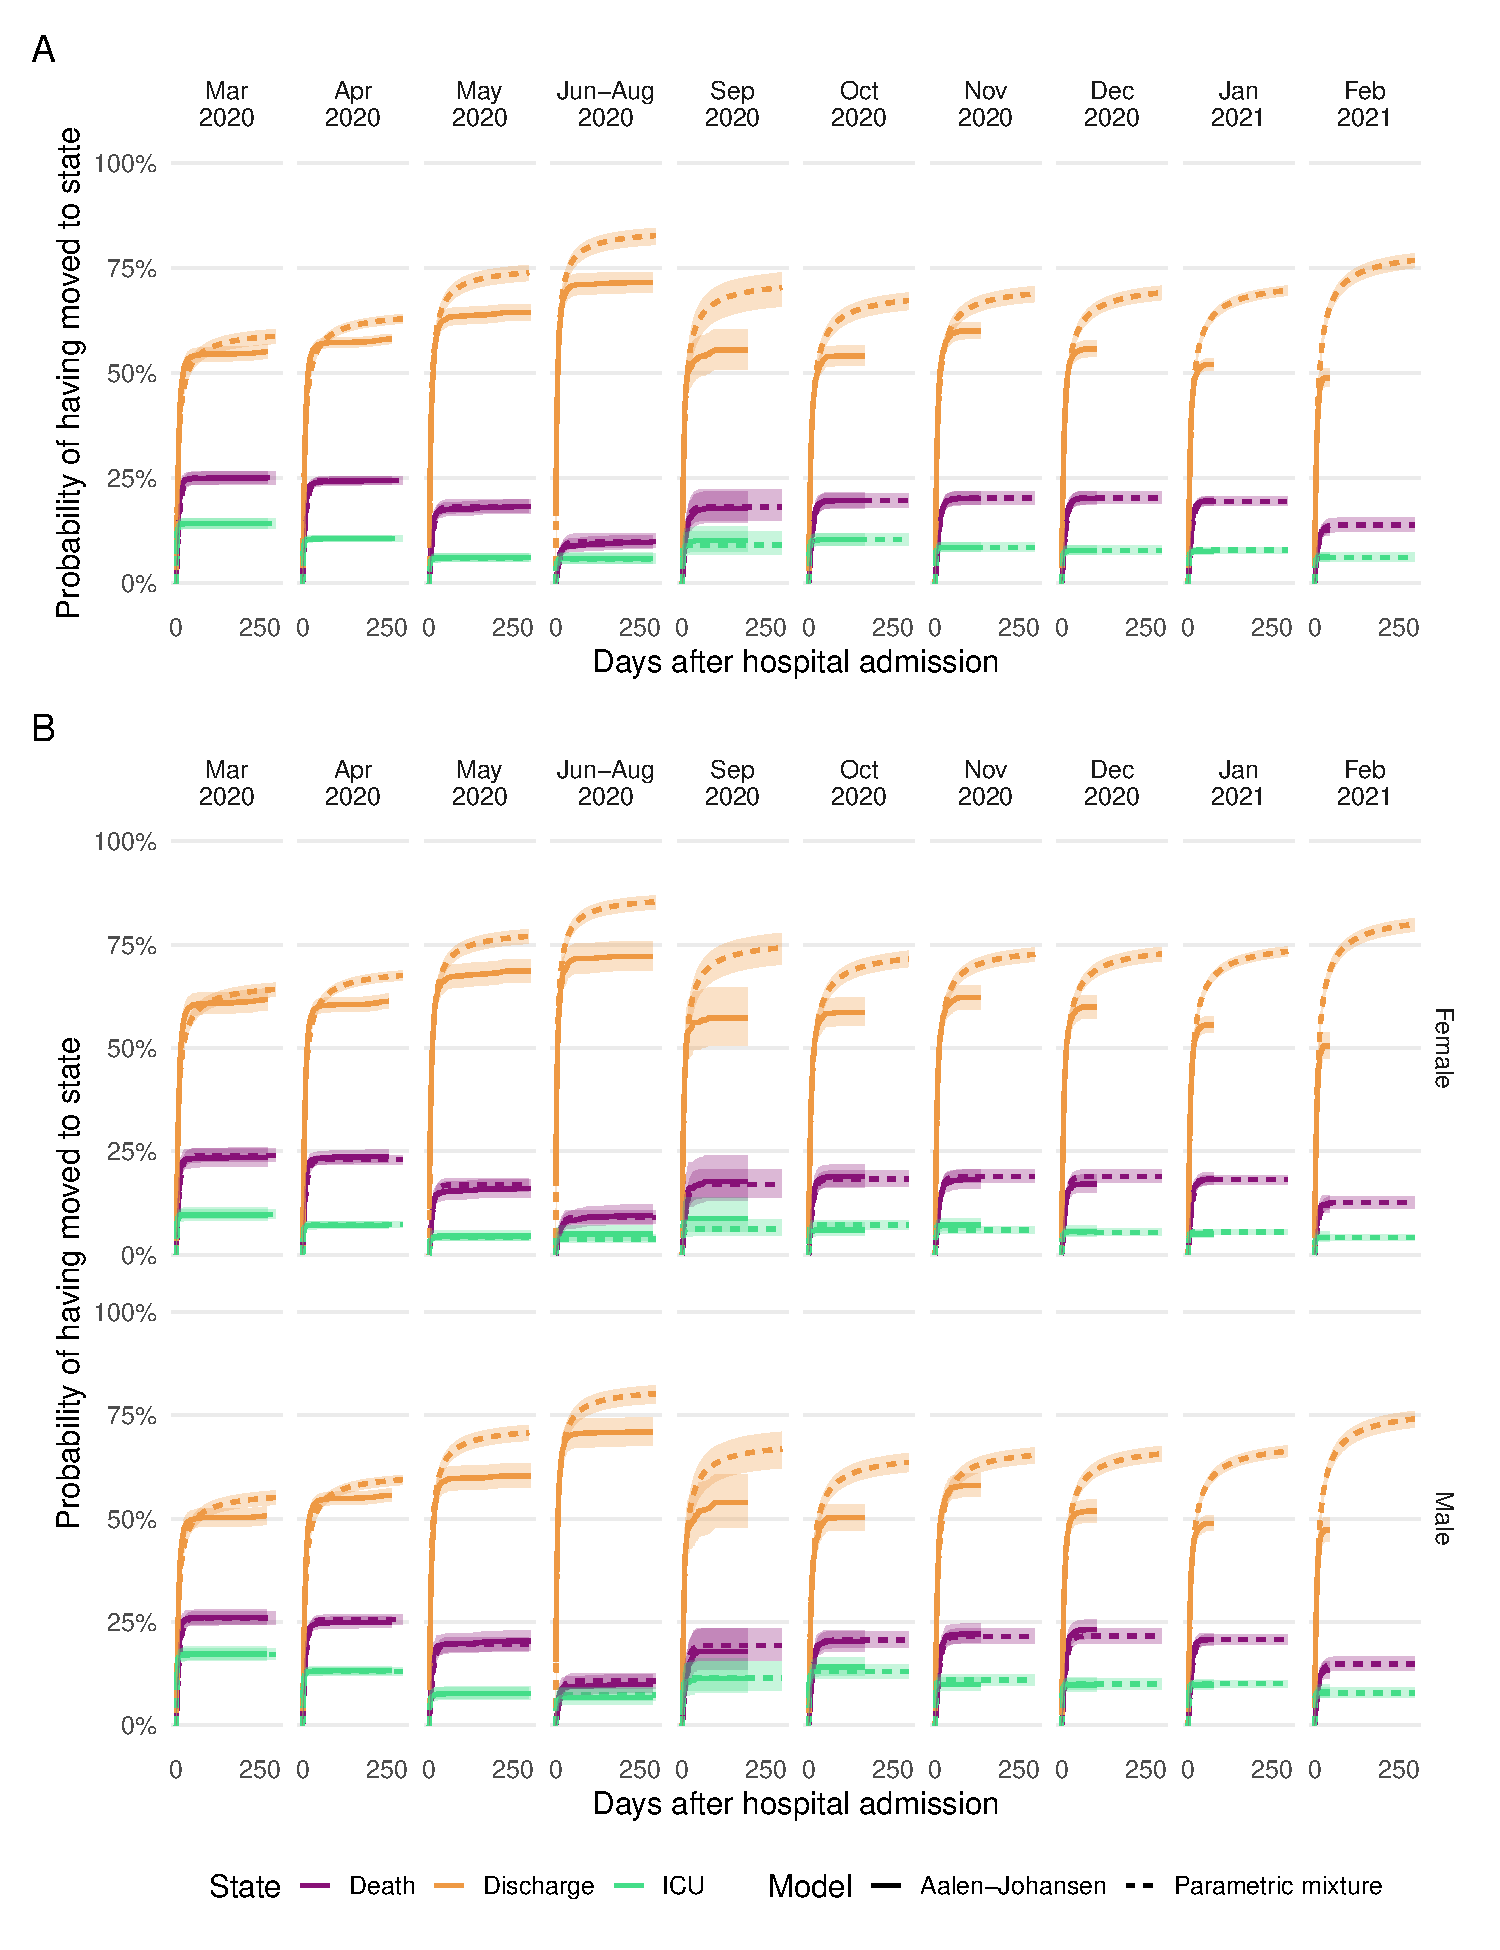
\includegraphics[width=\textwidth]{sari_gof_hosp.pdf}
    \caption[Goodness of fit for from Hospital sub-model in SARI-Watch data, March 2020 to February 2021]{Goodness of fit for sub-model (i) from Hospital, by month of admission (panel A), and sex (panel B) in SARI-Watch data, March 2020 to February 2021. Solid lines are Aalen-Johansen cumulative incidence curves, dashed lines are parametric mixture model estimates. Error bands are 95\% CIs, derived from 1000 simulation replicates.}\label{fig:sari-gof-hosp}
\end{figure}

\begin{figure}[htbp!]
    \centering
    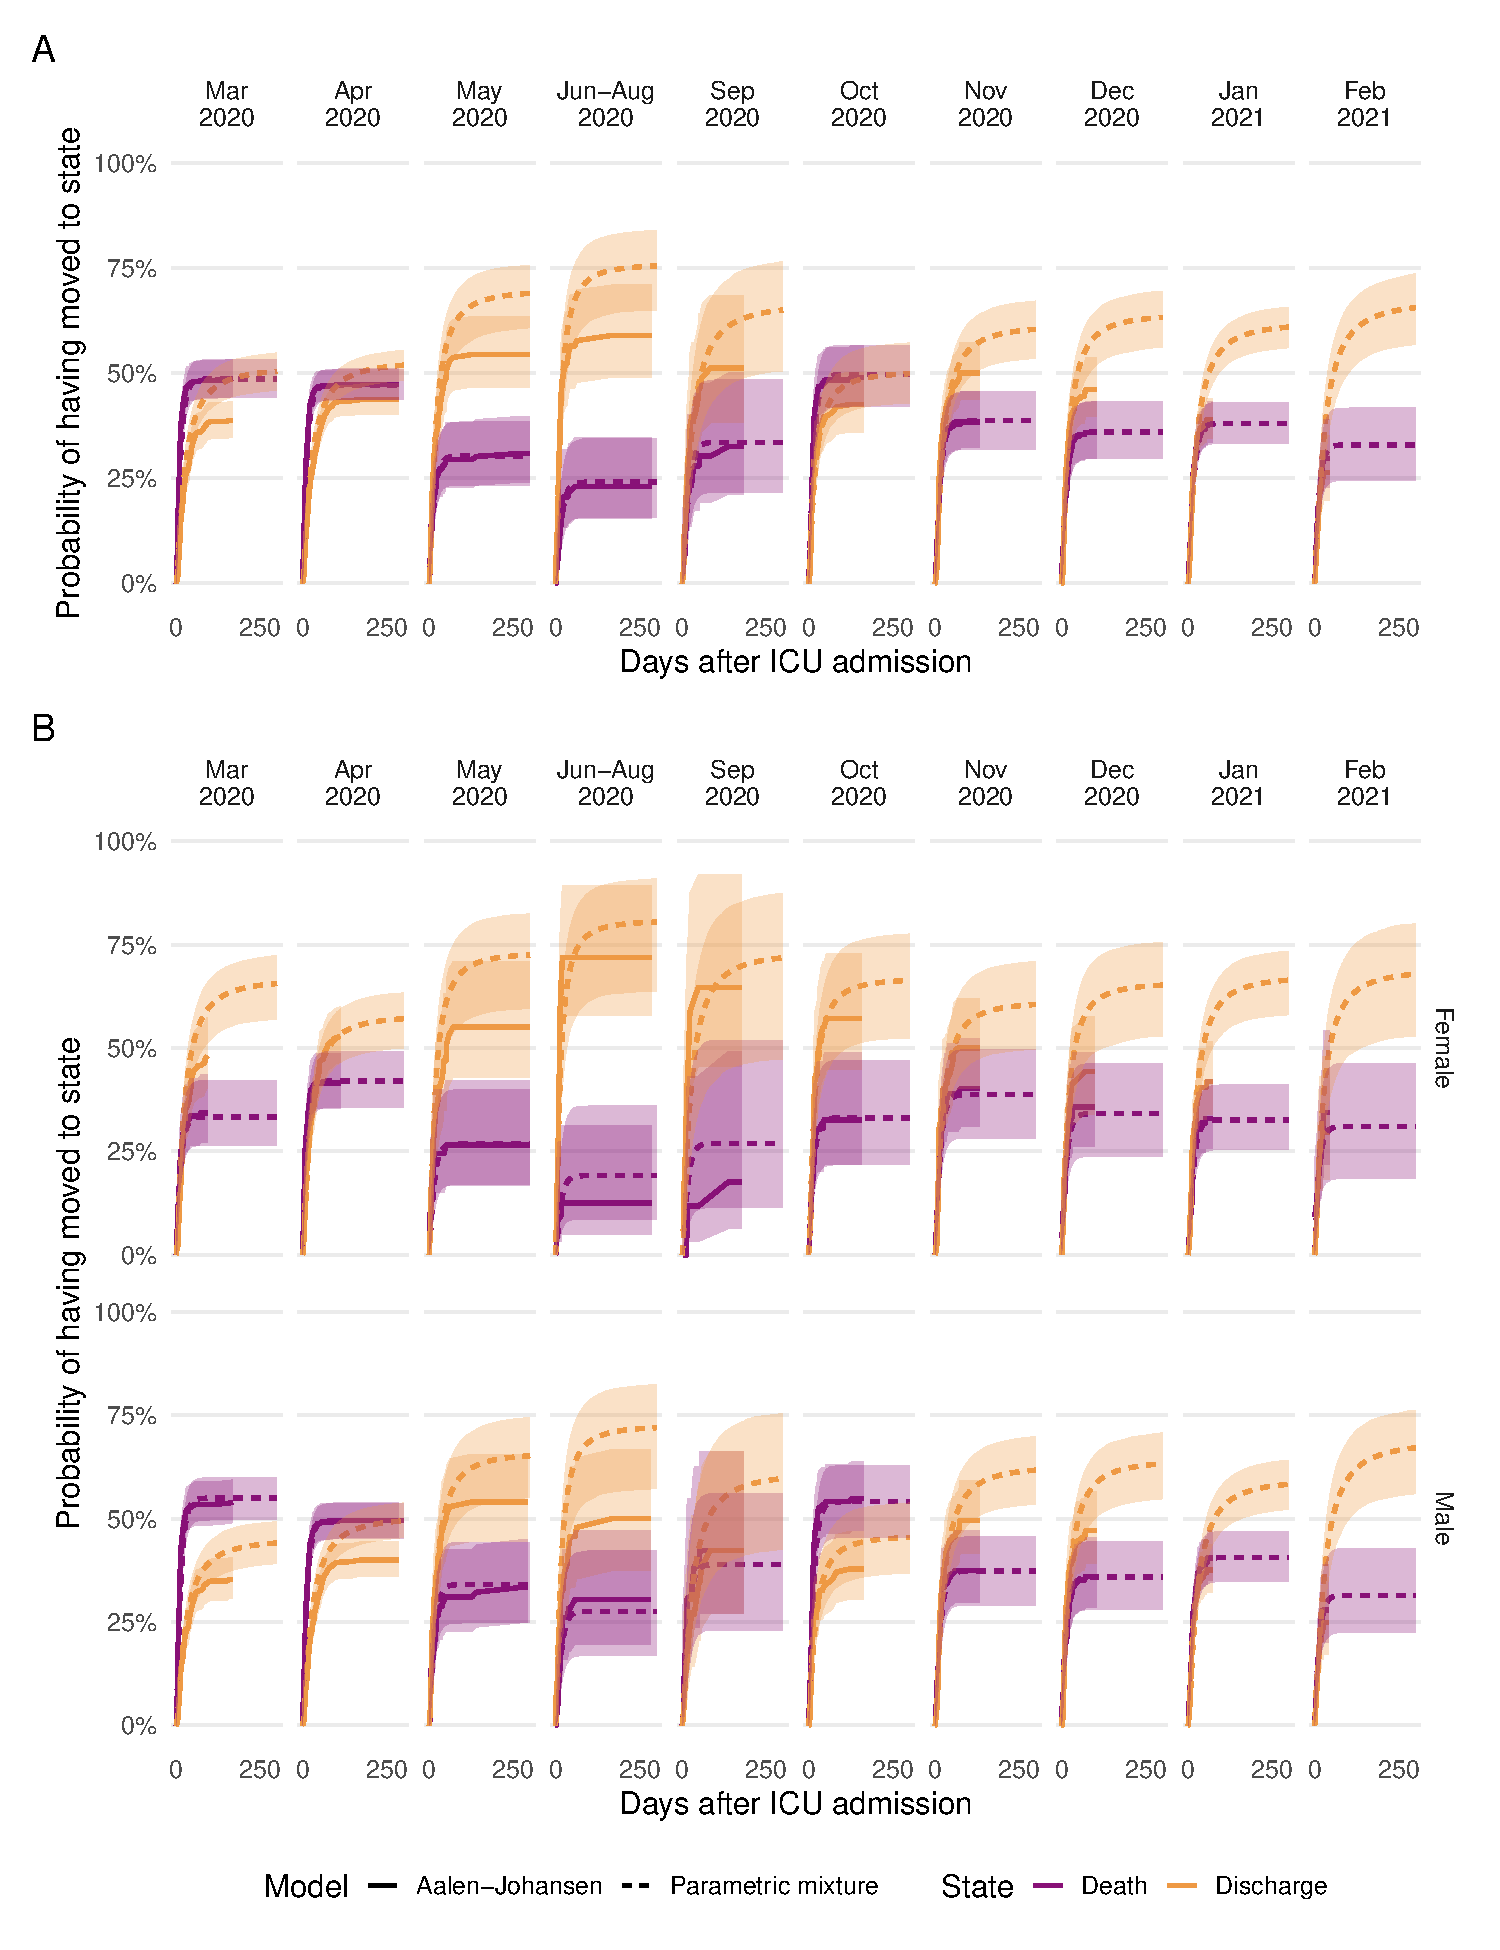
\includegraphics[width=\textwidth]{sari_gof_icu.pdf}
    \caption[Goodness of fit for from ICU sub-model in SARI-Watch data, March 2020 to February 2021]{Goodness of fit for sub-model (ii) from ICU, by month of admission (panel A), and sex (panel B) in SARI-Watch data, March 2020 to February 2021. Solid lines are Aalen-Johansen cumulative incidence curves, dashed lines are parametric mixture model estimates. Error bands are 95\% CIs, derived from 1000 simulation replicates.}\label{fig:sari-gof-icu}
\end{figure}

\subsection{Outcomes following ICU admission}\label{appendix:sari-icu}

The estimated probability of death among patients admitted to critical care by month of admission, sex, age group, and number of comorbidities is shown in Figure~\ref{fig:sari-icu-prob}, panels A--D. The probability of death following ICU admission fell from \var{sari_icu_death_mar} in March 2020 to \var{sari_icu_death_jun} in June-August 2020, increased to \var{sari_icu_death_oct} in October and plateaued at around \var{sari_icu_death_novdec} between November and December 2021. The probability of death following ICU admission was estimated to be greater among older patients compared to younger patients, although confidence intervals are wide for these smaller sub-groups.

\begin{figure}[htbp!]
    \centering
    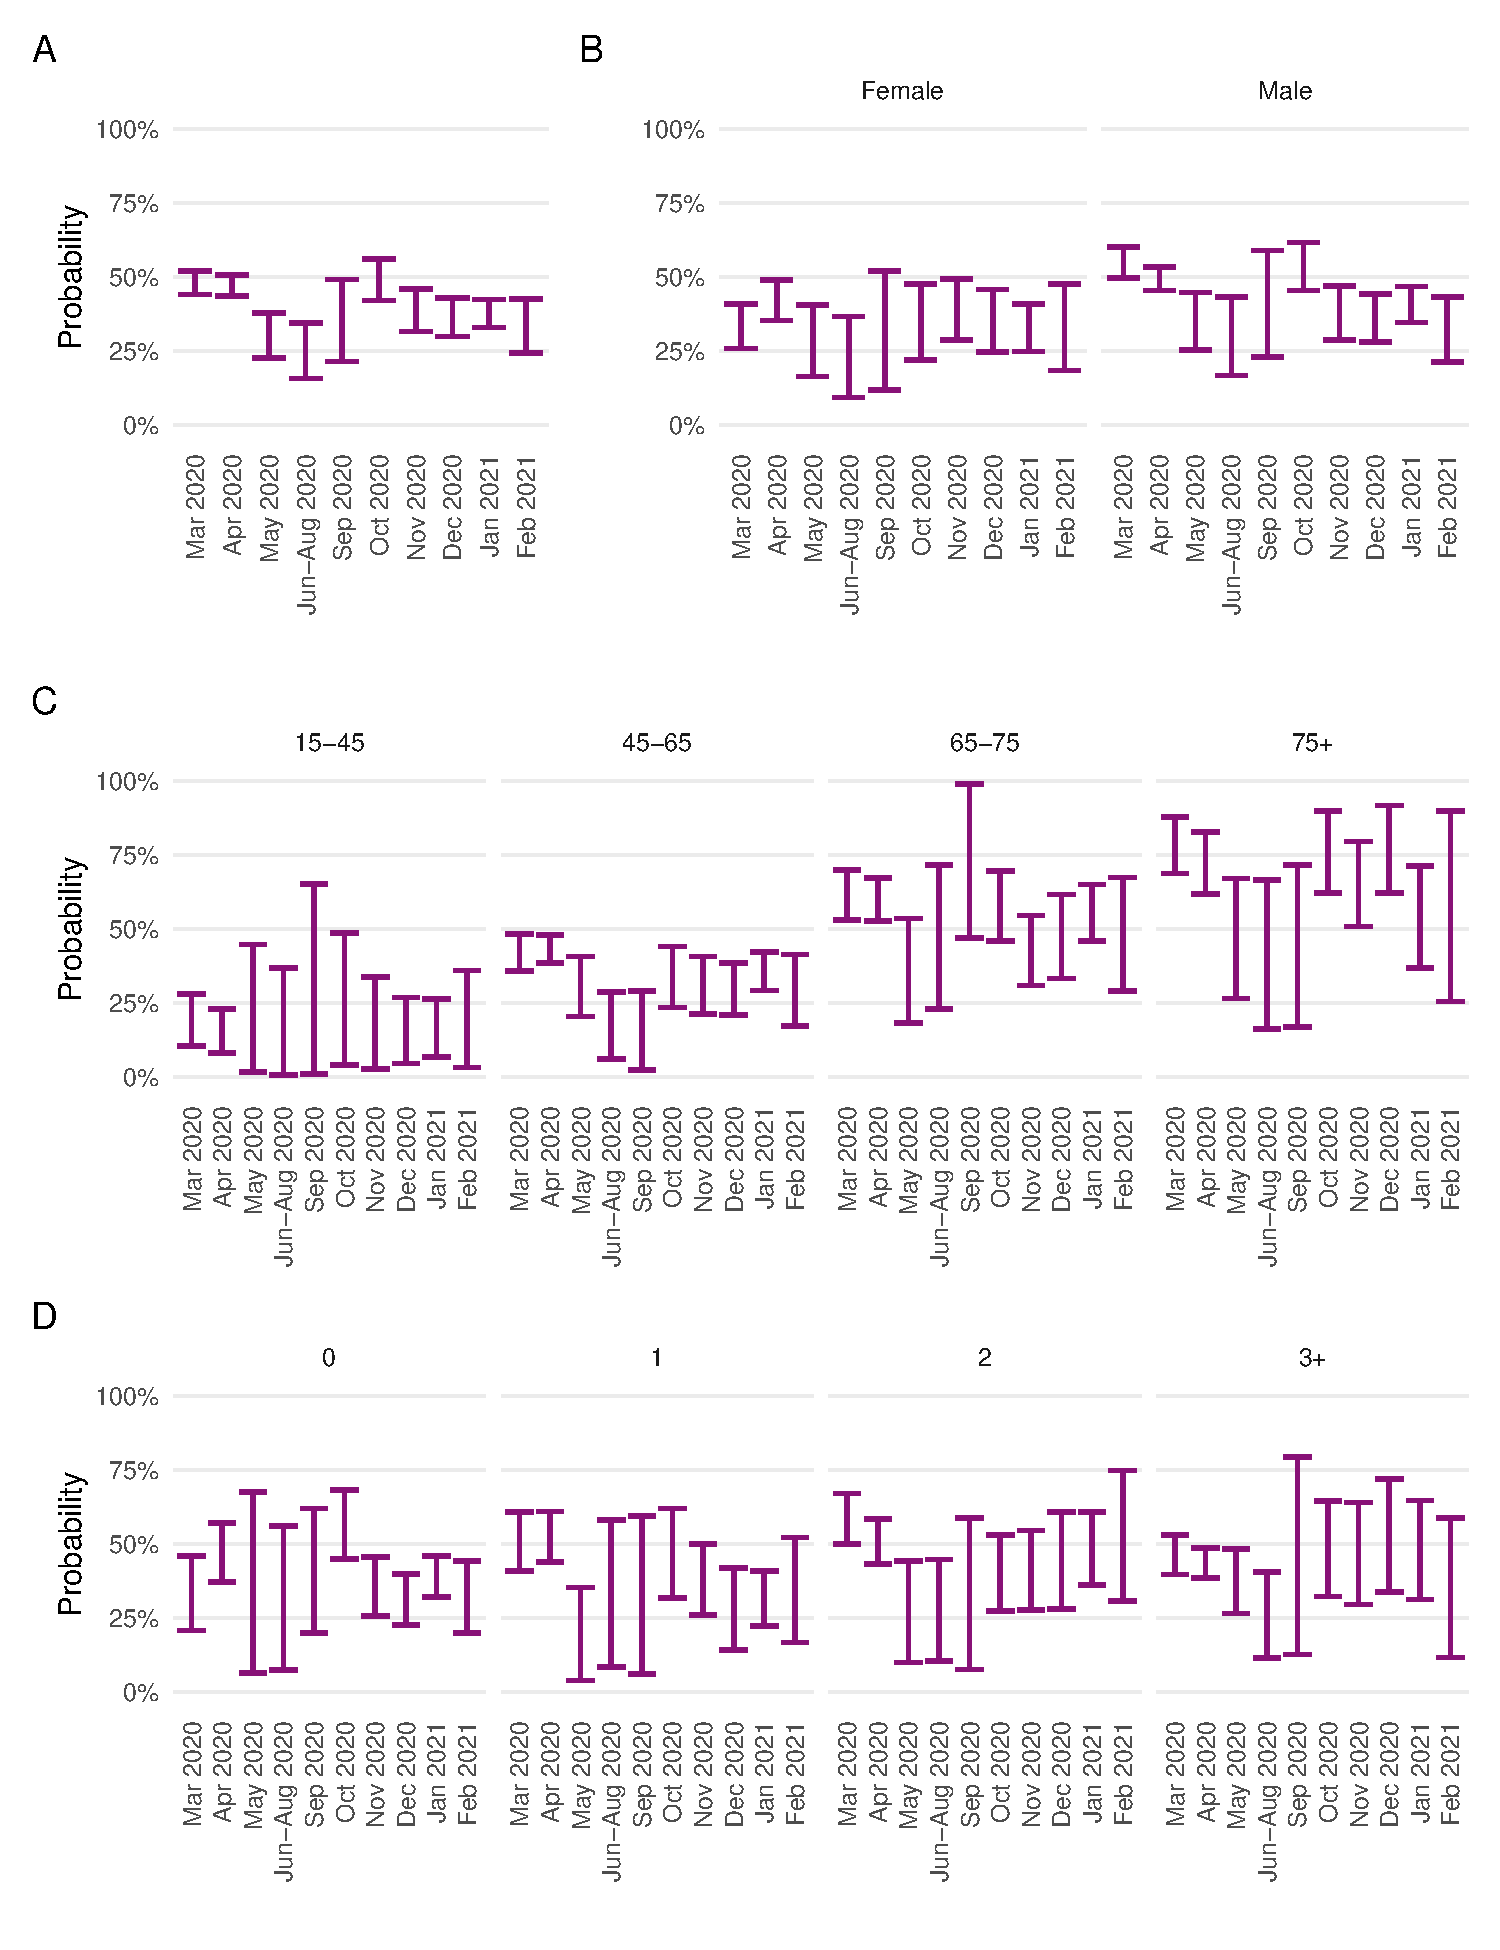
\includegraphics[width=\textwidth]{sari_icu_prob.pdf}
    \caption[Probability of death following ICU admission in SARI-Watch data, March 2020 to February 2021]{Probability of death following ICU admission, by month of admission (panel A), sex (panel B), age group (panel C), and number of comorbidities (panel D) in SARI-Watch data, March 2020 to February 2021. Error bands are 95\% CIs to represent uncertainty in the estimated probability.}\label{fig:sari-icu-prob}
\end{figure}

Figure~\ref{fig:sari-med-time-icu}, panels A--D, shows lengths of stay in ICU by month of admission, sex, age group, and number of comorbidities. Compared to non-critical care patients, those admitted to critical care spent longer in hospital. Median length of stay in ICU prior to discharge initially reduced from \var{sari_los_icu_disc_mar} in March 2020 to \var{sari_los_icu_disc_jun} in June-August 2020, then increased to \var{sari_los_icu_disc_dec} in December 2020. Median length of stay in ICU prior to death showed less variability over time, ranging between \var{sari_los_icu_death} days.

\begin{figure}[htbp!]
    \centering
    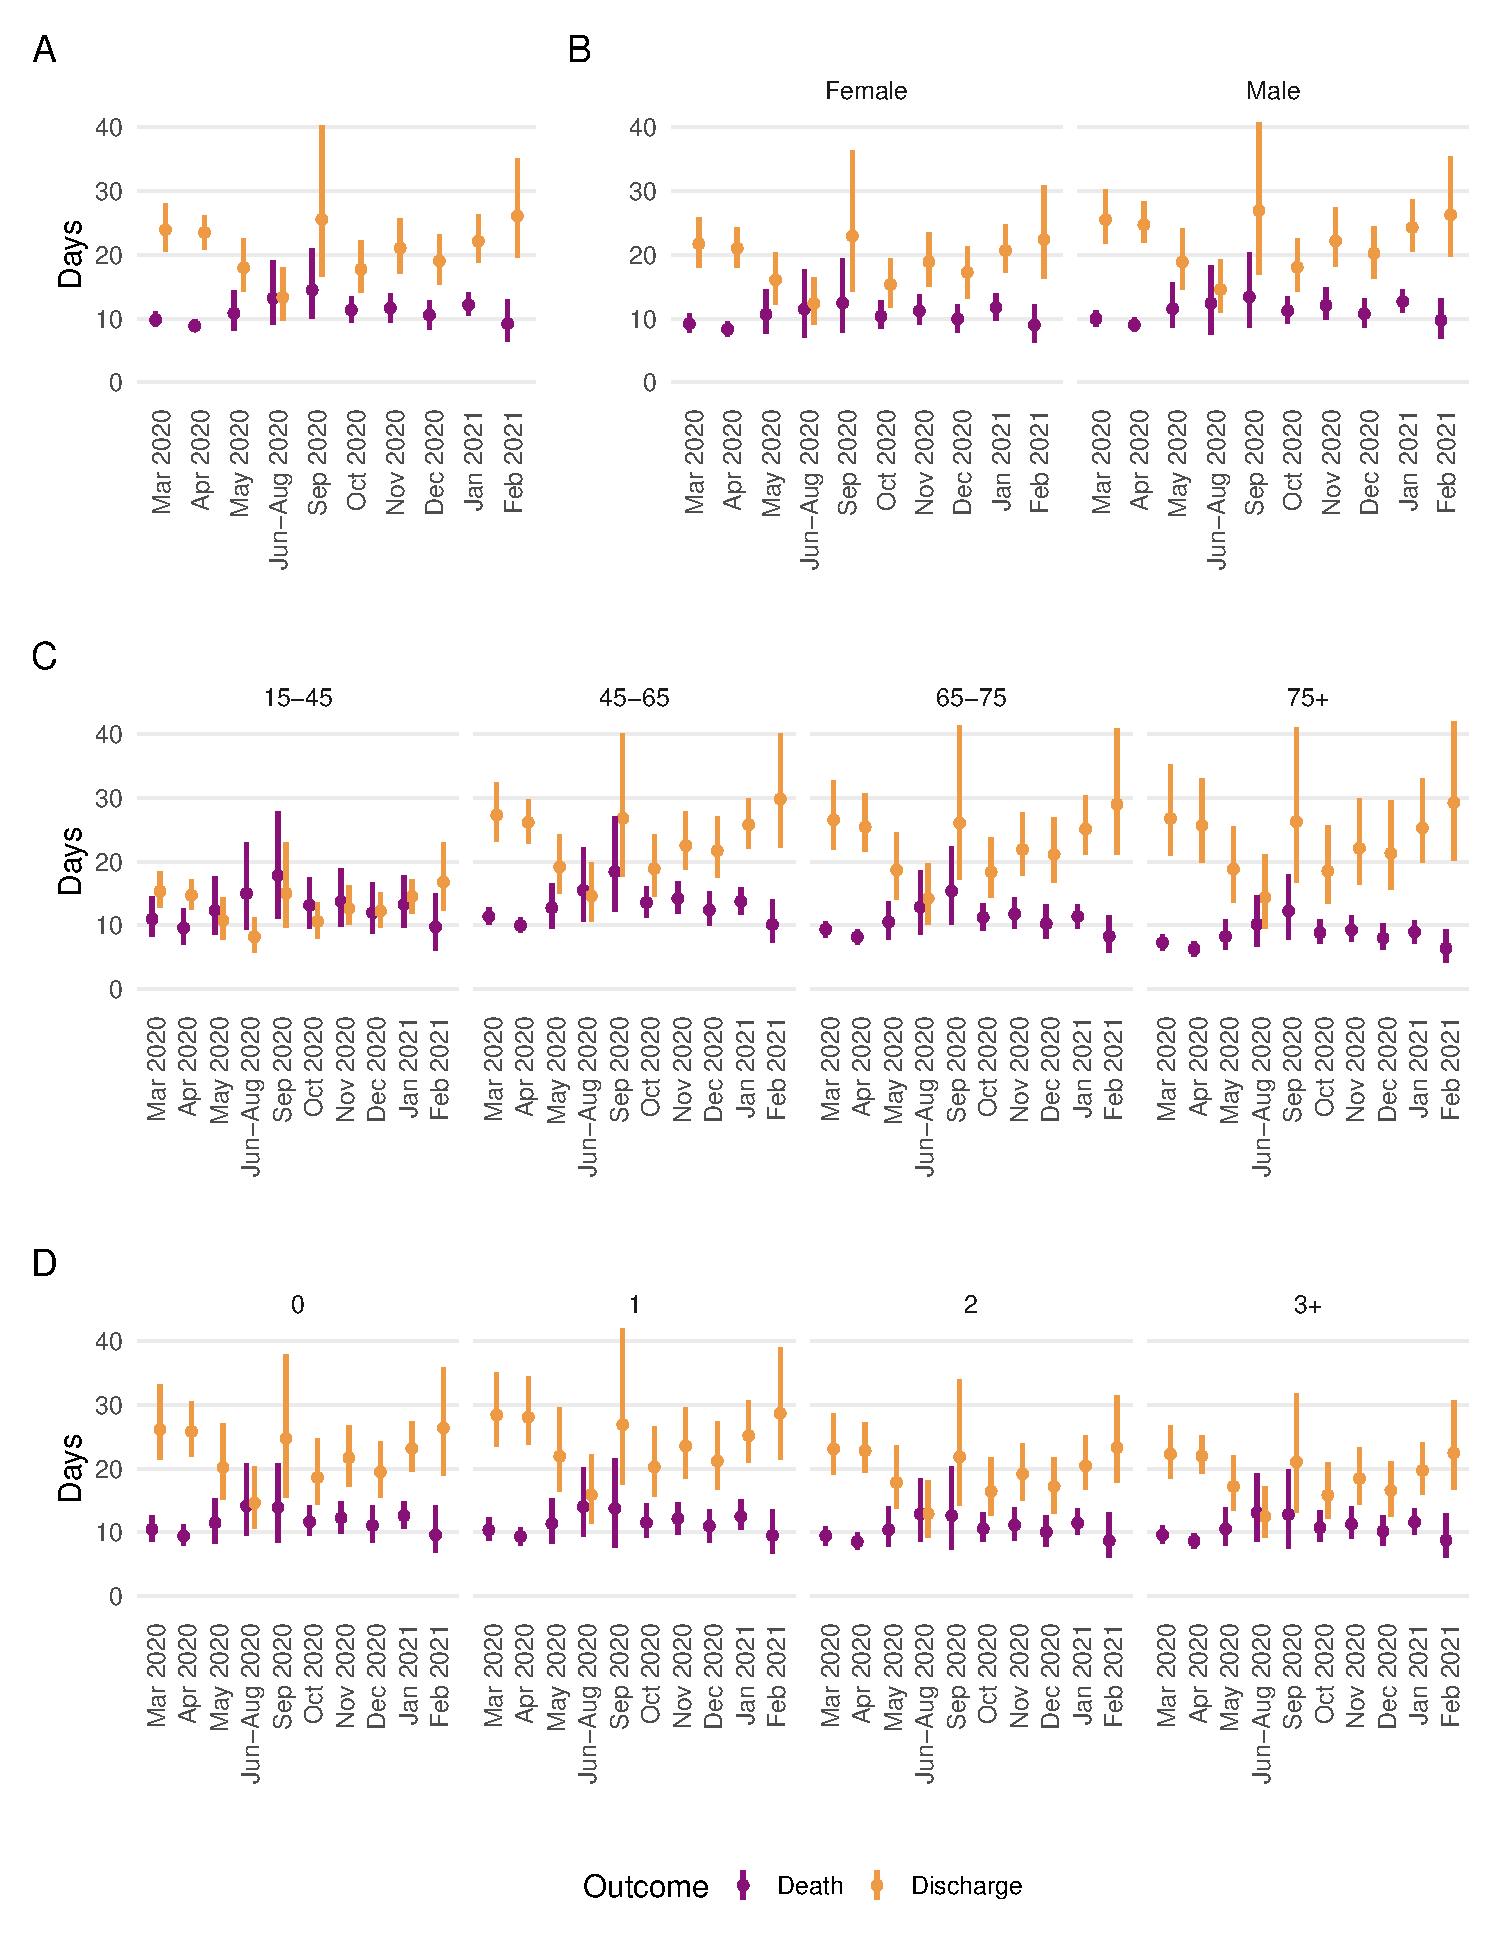
\includegraphics[width=\textwidth]{sari_med_time_icu.pdf}
    \caption[Estimated median time to event following ICU admission in SARI-Watch data, March 2020 to February 2021]{Estimated median time to event following ICU admission in SARI-Watch data, by month of admission (panel A), sex (panel B), age group (panel C), and number of comorbidities (panel D), March 2020 to February 2021. Line ranges are 95\% CIs around the median.}\label{fig:sari-med-time-icu}
\end{figure}

\clearpage

\section{Post-vaccine hospitalised severity}

\subsection{Weighted median with weighted ties}\label{sec:weighted-median}

For the $n$ elements in $\bm{x} = (x_1, x_2, \ldots, x_n)$ with positive weights $\bm{w} = (w_1, w_2, \ldots, w_n)$ and $S = \sum_n w_n$, the weighted median is the element $x_k$ where~\parencite{Cormen2022-pi}:
%
\begin{align*}
    \sum_{i<k} w_i & \leq \frac{S}{2} \\
    \sum_{i>k} w_i & \leq \frac{S}{2}
\end{align*}

When ties occur between two values $x_k$ which satisfy the weighted median criteria, the median is a weighted average of the two values, weighted by the sum of weights for all values $x_i \leq x_k$, and $x_i \geq x_k$, respectively.

\begingroup\footnotesize

\begin{longtable}[t]{lccc}
\caption{\label{tab:sus_characteristics}Characteristics of the study population compared with all people hospital-onset COVID-19, and all people with PCR-confirmed community-acquired COVID-19 in England.}\\
\toprule
\textbf{Characteristic} & \makecell[c]{\textbf{Study population}\ \ \\ \textbf{(hospitalised for}\ \ \\ \textbf{COVID-19}\ \ \\ \textbf{in England)}\ \ \\N = 590,313} & \makecell[c]{\textbf{All people with}\ \ \\ \textbf{hospital-onset}\ \ \\ \textbf{COVID-19}\ \ \\ \textbf{in England}\ \ \\N = 209,139} & \makecell[c]{\textbf{All people with}\ \ \\ \textbf{PCR-confirmed,}\ \ \\ \textbf{community-acquired}\ \ \\ \textbf{COVID-19 in England}\ \ \\N = 6,617,362}\\
\midrule
Age group &  &  & \\
\hspace{1em}0--14 & 19,186 (3.3\%) & 2,635 (1.3\%) & 892,380 (13\%)\\
\hspace{1em}15--24 & 28,936 (4.9\%) & 4,437 (2.1\%) & 1,264,528 (19\%)\\
\hspace{1em}25--44 & 122,390 (21\%) & 13,764 (6.6\%) & 2,244,393 (34\%)\\
\hspace{1em}45--64 & 154,594 (26\%) & 33,209 (16\%) & 1,560,517 (24\%)\\
\hspace{1em}65--74 & 90,037 (15\%) & 36,537 (17\%) & 301,440 (4.6\%)\\
\hspace{1em}75--84 & 101,578 (17\%) & 59,892 (29\%) & 198,209 (3.0\%)\\
\hspace{1em}85+ & 73,592 (12\%) & 58,665 (28\%) & 155,895 (2.4\%)\\
Sex &  &  & \\
\hspace{1em}Male & 289,085 (49\%) & 108,709 (52\%) & 3,152,281 (48\%)\\
\hspace{1em}Female & 301,228 (51\%) & 100,430 (48\%) & 3,465,081 (52\%)\\
Ethnicity &  &  & \\
\hspace{1em}White & 444,615 (75\%) & 185,426 (89\%) & 5,100,779 (77\%)\\
\hspace{1em}Asian & 58,411 (9.9\%) & 9,877 (4.7\%) & 740,301 (11\%)\\
\hspace{1em}Black & 33,961 (5.8\%) & 6,362 (3.0\%) & 278,844 (4.2\%)\\
\hspace{1em}Mixed/Other/Unknown & 41,386 (7.0\%) & 7,474 (3.6\%) & 497,438 (7.5\%)\\
\hspace{1em}Prefer not to say & 11,940 (2.0\%) & 0 (0\%) & 0 (0\%)\\
Region of residence &  &  & \\
\hspace{1em}London & 104,850 (18\%) & 28,779 (14\%) & 1,078,524 (16\%)\\
\hspace{1em}East Midlands & 51,147 (8.7\%) & 18,774 (9.0\%) & 586,490 (8.9\%)\\
\hspace{1em}East of England & 59,735 (10\%) & 22,809 (11\%) & 679,080 (10\%)\\
\hspace{1em}North East & 33,809 (5.7\%) & 9,416 (4.5\%) & 376,501 (5.7\%)\\
\hspace{1em}North West & 94,658 (16\%) & 42,276 (20\%) & 1,056,101 (16\%)\\
\hspace{1em}South East & 76,913 (13\%) & 28,819 (14\%) & 887,347 (13\%)\\
\hspace{1em}South West & 48,448 (8.2\%) & 12,880 (6.2\%) & 496,337 (7.5\%)\\
\hspace{1em}West Midlands & 66,495 (11\%) & 24,544 (12\%) & 733,204 (11\%)\\
\hspace{1em}Yorkshire and Humber & 54,258 (9.2\%) & 20,842 (10.0\%) & 723,778 (11\%)\\
\multicolumn{3}{l}{Index of Multiple Deprivation}  & \\
\hspace{1em}Most deprived & 159,904 (27\%) & 51,314 (25\%) & 1,564,566 (24\%)\\
\hspace{1em}2nd quintile & 133,835 (23\%) & 44,996 (22\%) & 1,440,738 (22\%)\\
\hspace{1em}3rd quintile & 111,840 (19\%) & 40,584 (19\%) & 1,288,334 (19\%)\\
\hspace{1em}4th quintile & 99,313 (17\%) & 38,418 (18\%) & 1,210,037 (18\%)\\
\hspace{1em}Least deprived & 85,421 (14\%) & 33,827 (16\%) & 1,113,687 (17\%)\\
Hospital outcome &  &  & \\
\hspace{1em}Death & 81,343 (14\%) & 69,469 (33\%) & -\\
\hspace{1em}Discharge & 507,254 (86\%) & 107,878 (52\%) & -\\
\hspace{1em}Right-censored in hospital & 1,716 (0.3\%) & 31,792 (15\%) & -\\
Month of hospital admission &  &  & \\
\hspace{1em}Mar 2020 & 18,285 (3.1\%) & - & -\\
\hspace{1em}Apr 2020 & 36,524 (6.2\%) & - & -\\
\hspace{1em}May 2020 & 10,471 (1.8\%) & - & -\\
\hspace{1em}Jun 2020 & 3,826 (0.6\%) & - & -\\
\hspace{1em}Jul 2020 & 1,506 (0.3\%) & - & -\\
\hspace{1em}Aug 2020 & 1,276 (0.2\%) & - & -\\
\hspace{1em}Sep 2020 & 5,175 (0.9\%) & - & -\\
\hspace{1em}Oct 2020 & 19,525 (3.3\%) & - & -\\
\hspace{1em}Nov 2020 & 29,932 (5.1\%) & - & -\\
\hspace{1em}Dec 2020 & 40,657 (6.9\%) & - & -\\
\hspace{1em}Jan 2021 & 77,186 (13\%) & - & -\\
\hspace{1em}Feb 2021 & 25,488 (4.3\%) & - & -\\
\hspace{1em}Mar 2021 & 7,941 (1.3\%) & - & -\\
\hspace{1em}Apr 2021 & 3,100 (0.5\%) & - & -\\
\hspace{1em}May 2021 & 2,260 (0.4\%) & - & -\\
\hspace{1em}Jun 2021 & 5,597 (0.9\%) & - & -\\
\hspace{1em}Jul 2021 & 20,340 (3.4\%) & - & -\\
\hspace{1em}Aug 2021 & 22,388 (3.8\%) & - & -\\
\hspace{1em}Sep 2021 & 19,510 (3.3\%) & - & -\\
\hspace{1em}Oct 2021 & 21,974 (3.7\%) & - & -\\
\hspace{1em}Nov 2021 & 20,707 (3.5\%) & - & -\\
\hspace{1em}Dec 2021 & 31,716 (5.4\%) & - & -\\
\hspace{1em}Jan 2022 & 54,310 (9.2\%) & - & -\\
\hspace{1em}Feb 2022 & 28,412 (4.8\%) & - & -\\
\hspace{1em}Mar 2022 & 42,885 (7.3\%) & - & -\\
\hspace{1em}Apr 2022 & 39,322 (6.7\%) & - & -\\
\multicolumn{3}{l}{Vaccination status at date of admission (January 2021 onwards)}  & \\
\hspace{1em}Unvaccinated & 367,082 (62\%) & - & -\\
\hspace{1em}<21 days after first dose & 14,385 (2.4\%) & - & -\\
\hspace{1em}$\leq$21 days after first dose & 20,711 (3.5\%) & - & -\\
\hspace{1em}$\geq$14 days after second dose & 119,559 (20\%) & - & -\\
\hspace{1em}$\geq$14 days after third dose & 68,576 (12\%) & - & -\\
Charlson comorbidity index &  &  & \\
\hspace{1em}0 & 232,646 (39\%) & - & -\\
\hspace{1em}1-2 & 227,174 (38\%) & - & -\\
\hspace{1em}3-4 & 85,131 (14\%) & - & -\\
\hspace{1em}5+ & 45,362 (7.7\%) & - & -\\
\multicolumn{3}{l}{Hospital load at time of admission (as proportion of busiest week)}  & \\
\hspace{1em}0-20\% & 120,259 (20\%) & - & -\\
\hspace{1em}20-40\% & 192,060 (33\%) & - & -\\
\hspace{1em}40-60\% & 123,943 (21\%) & - & -\\
\hspace{1em}60-80\% & 80,567 (14\%) & - & -\\
\hspace{1em}80-90\% & 34,308 (5.8\%) & - & -\\
\hspace{1em}90-100\% & 39,176 (6.6\%) & - & -\\
\bottomrule
\end{longtable}

\endgroup

\begin{figure}[htbp!]
    \centering
    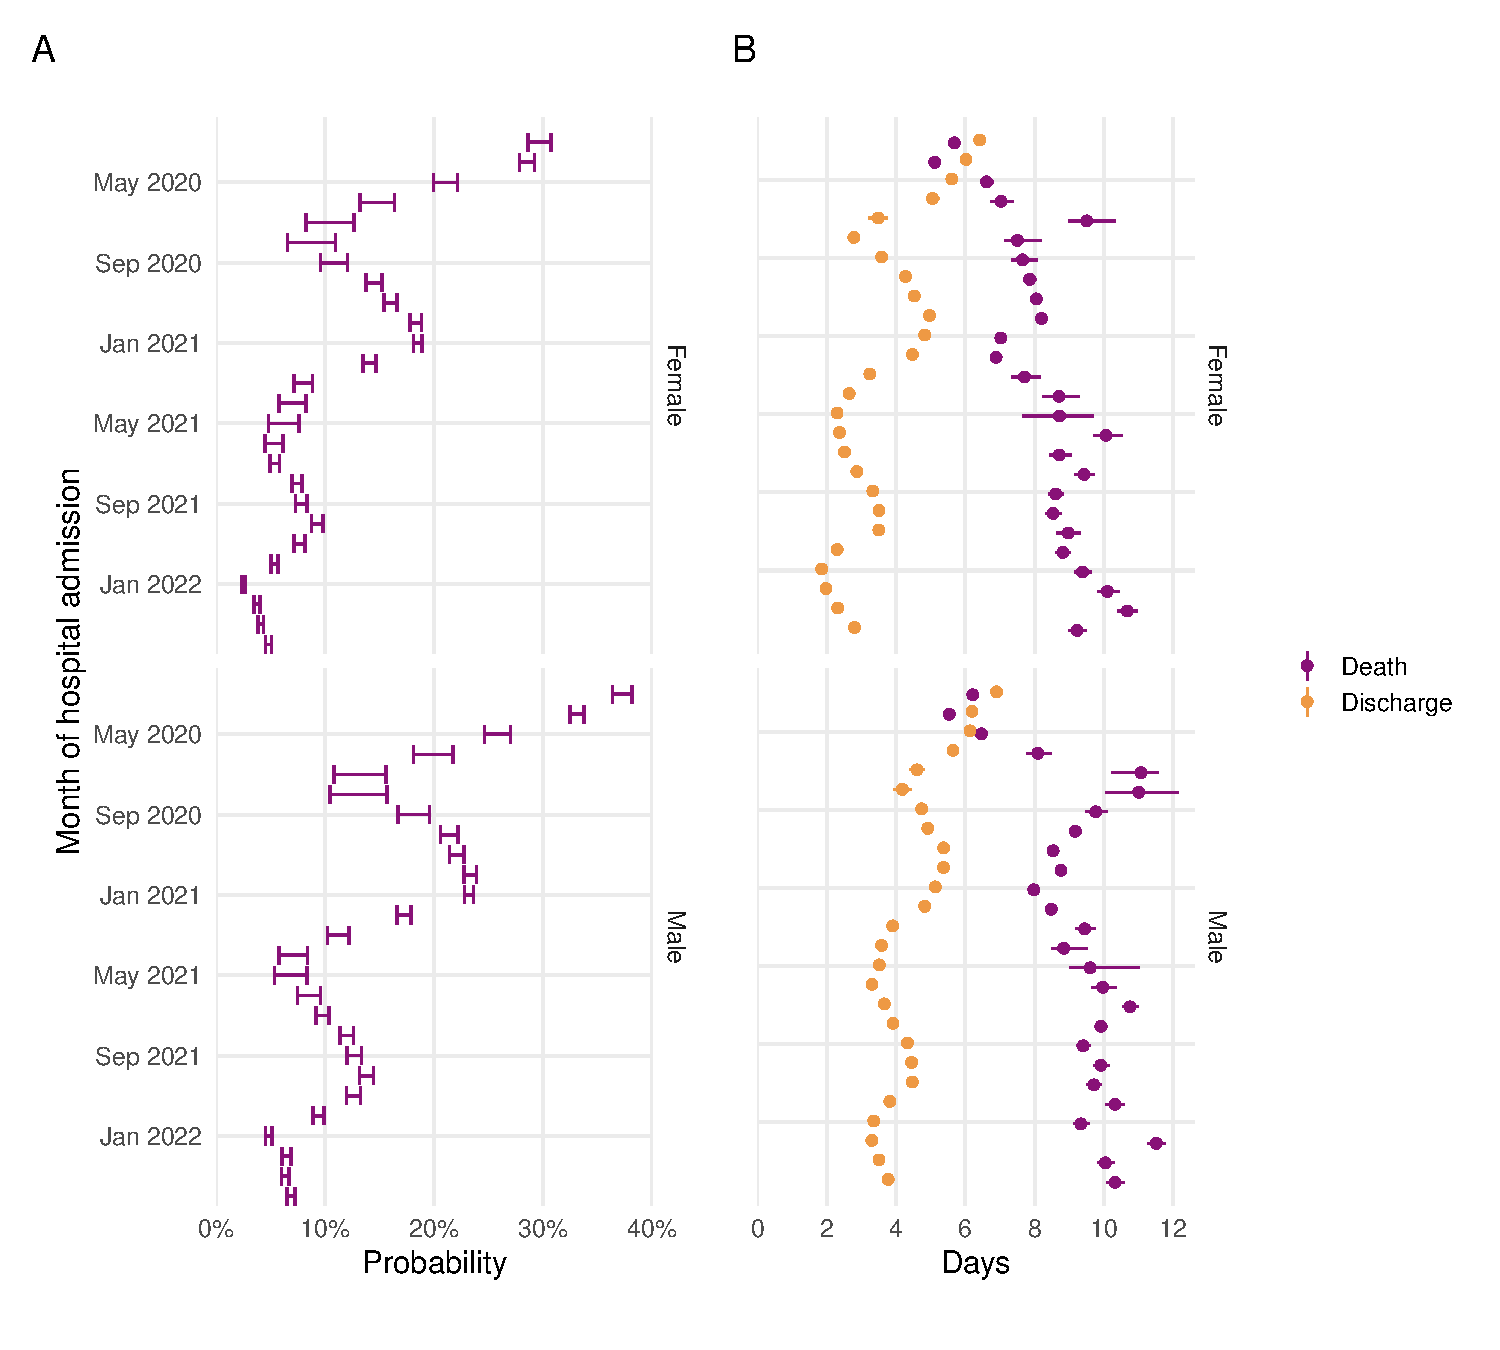
\includegraphics[width=\textwidth]{hfr_month_sex.pdf}
    \caption[Hospitalised fatality risk and median length of stay by month of admission and sex in SUS data, March 2020 to April 2022]{Hospitalised fatality risk (panel A) and median length of stay (panel B) by month of admission and sex in SUS data, March 2020 to April 2022. Unadjusted for other covariates. Error bars and line ranges are 95\% CIs.}
\end{figure}

\begin{figure}[htbp!]
    \centering
    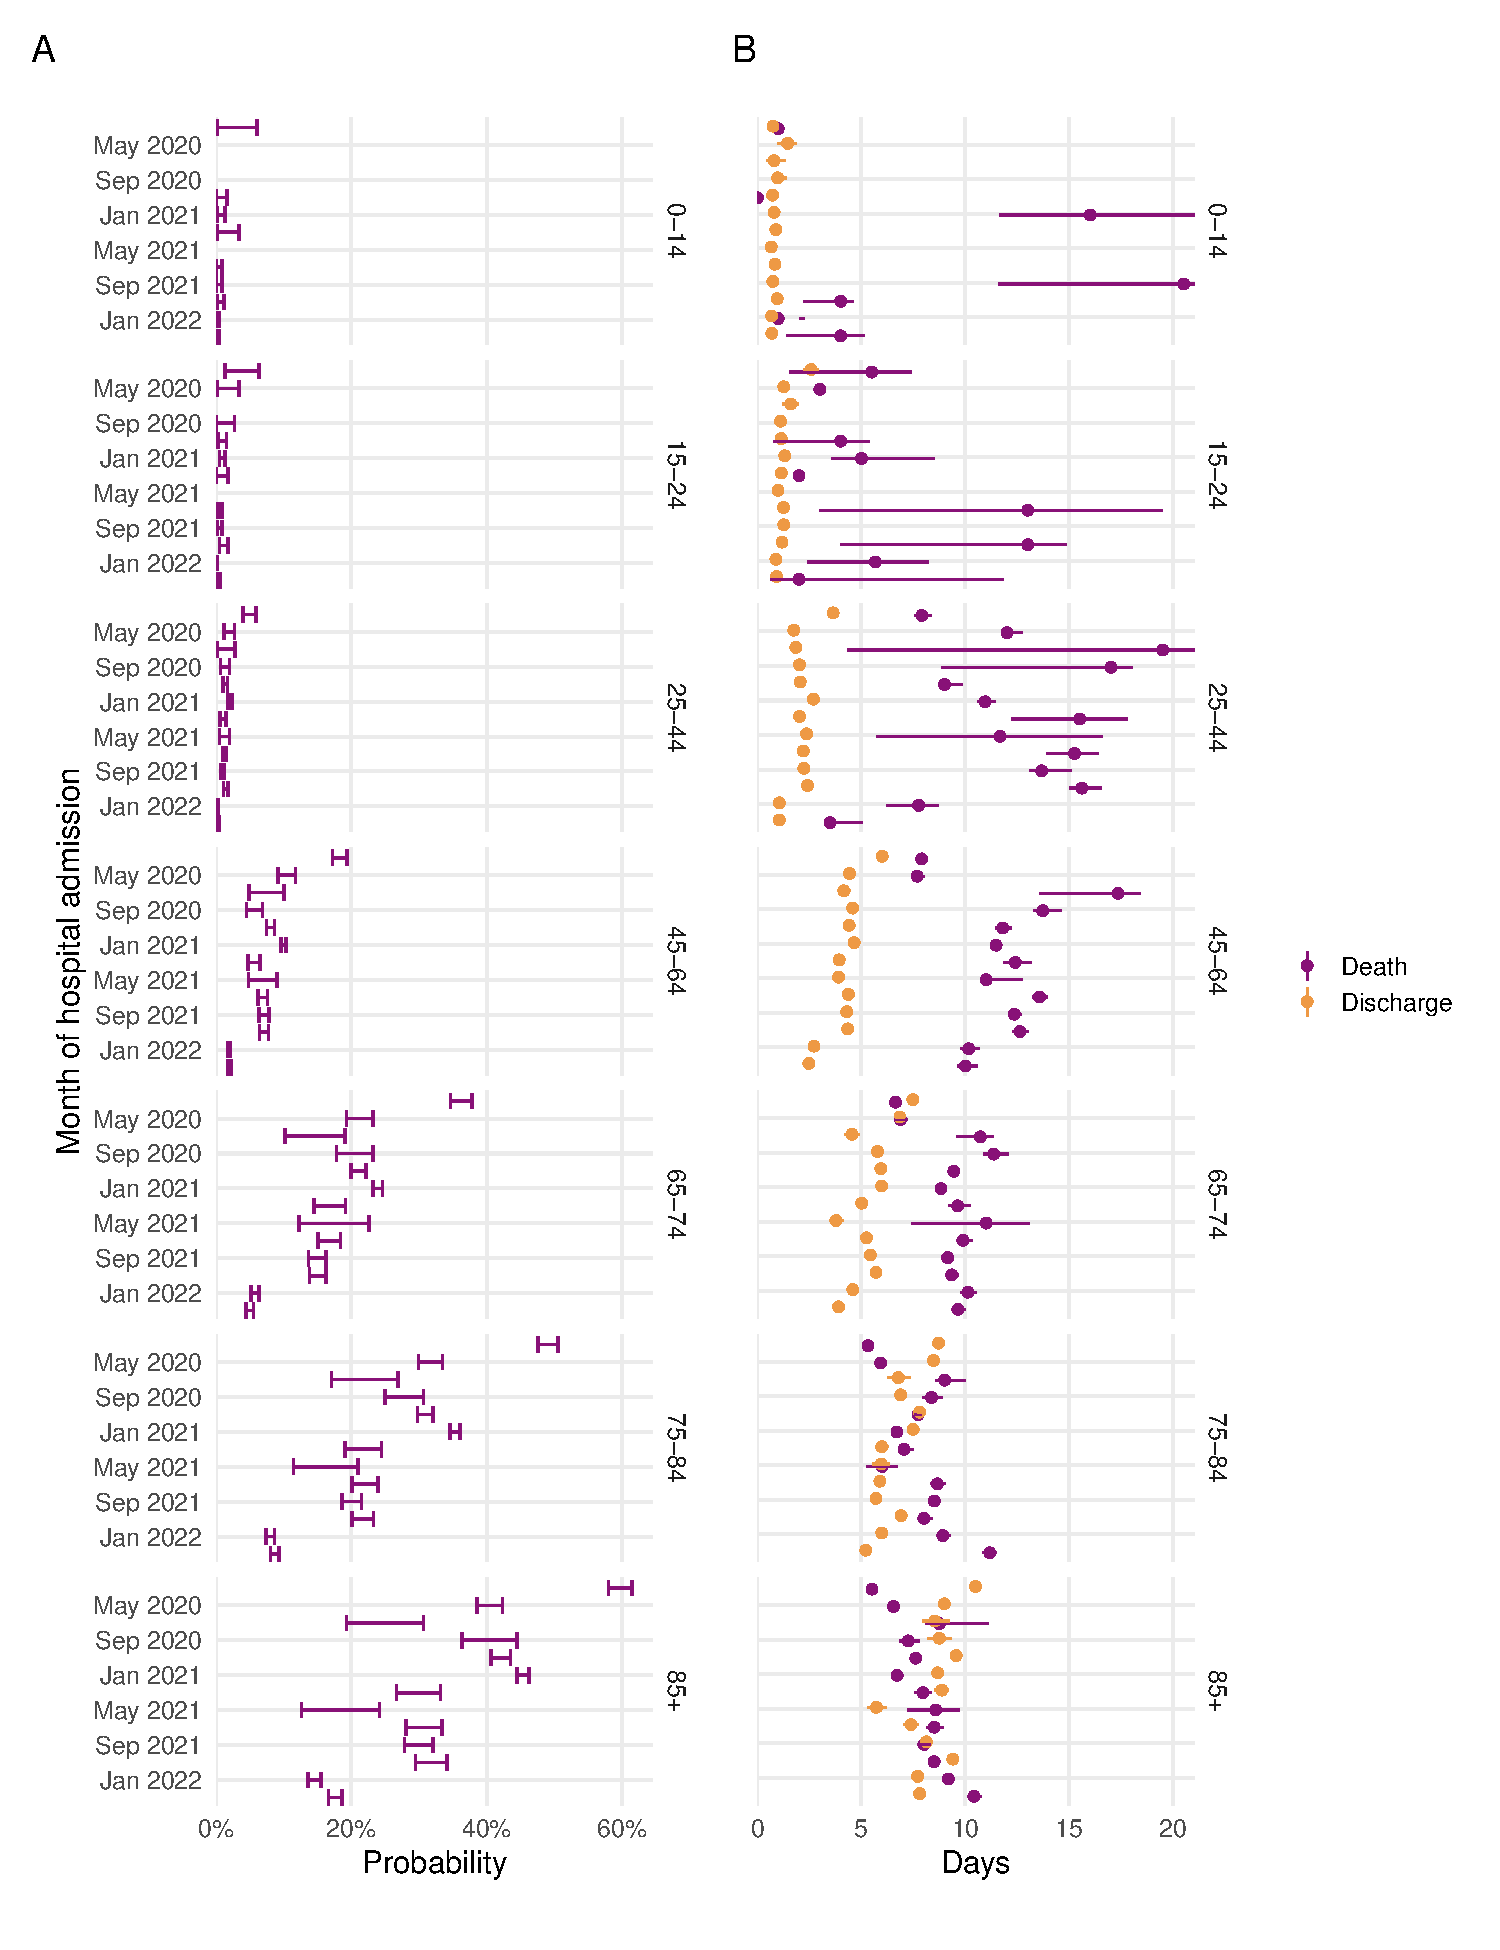
\includegraphics[width=\textwidth]{hfr_month_age.pdf}
    \caption[Hospitalised fatality risk and median length of stay by month of admission and age group in SUS data, March 2020 to April 2022]{Hospitalised fatality risk (panel A) and median length of stay (panel B) by month of admission and age group in SUS data, March 2020 to April 2022. Unadjusted for other covariates. Error bars and line ranges are 95\% CIs.}\label{fig:hfr-month-age}
\end{figure}

\begin{figure}[htbp!]
    \centering
    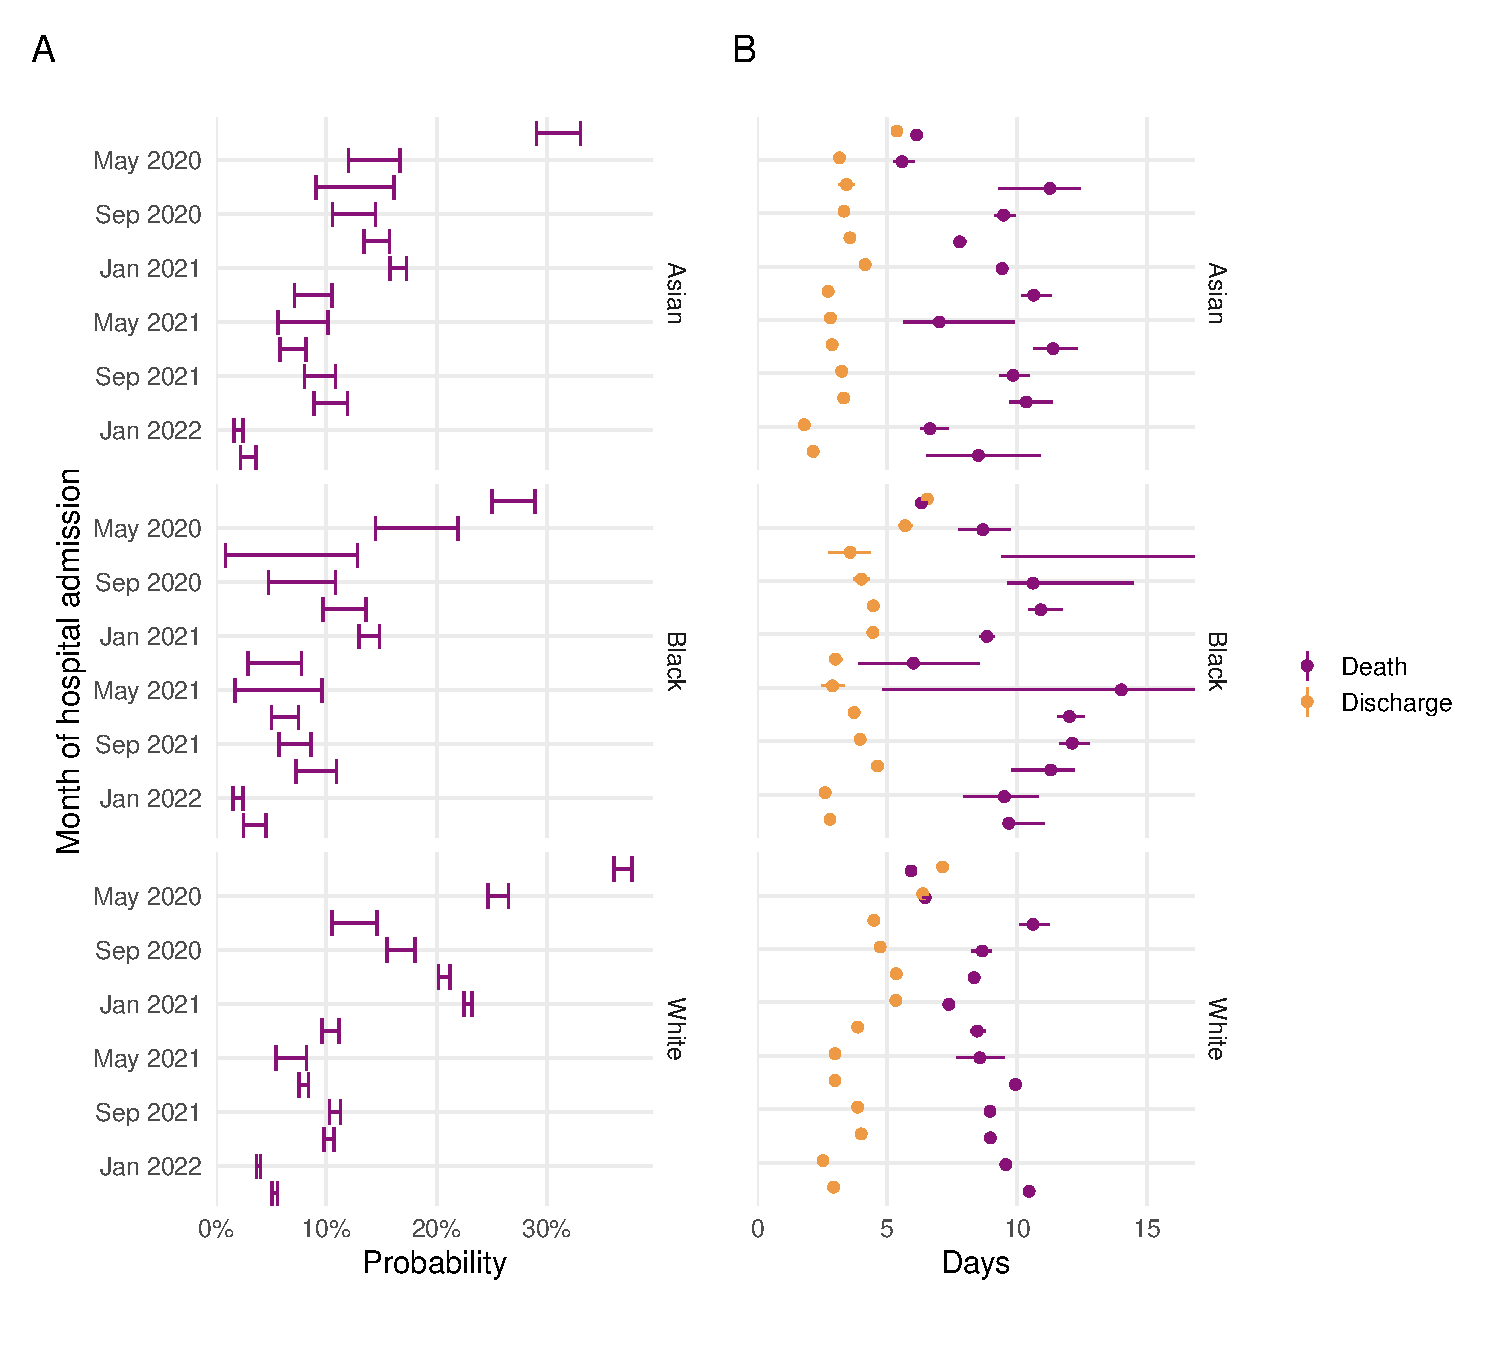
\includegraphics[width=\textwidth]{hfr_month_ethn.pdf}
    \caption[Hospitalised fatality risk and median length of stay by month of admission and ethnicity in SUS data, March 2020 to April 2022]{Hospitalised fatality risk (panel A) and median length of stay (panel B) by month of admission and ethnicity in SUS data, March 2020 to April 2022. Unadjusted for other covariates. Error bars and line ranges are 95\% CIs.}
\end{figure}

\begin{figure}[htbp!]
    \centering
    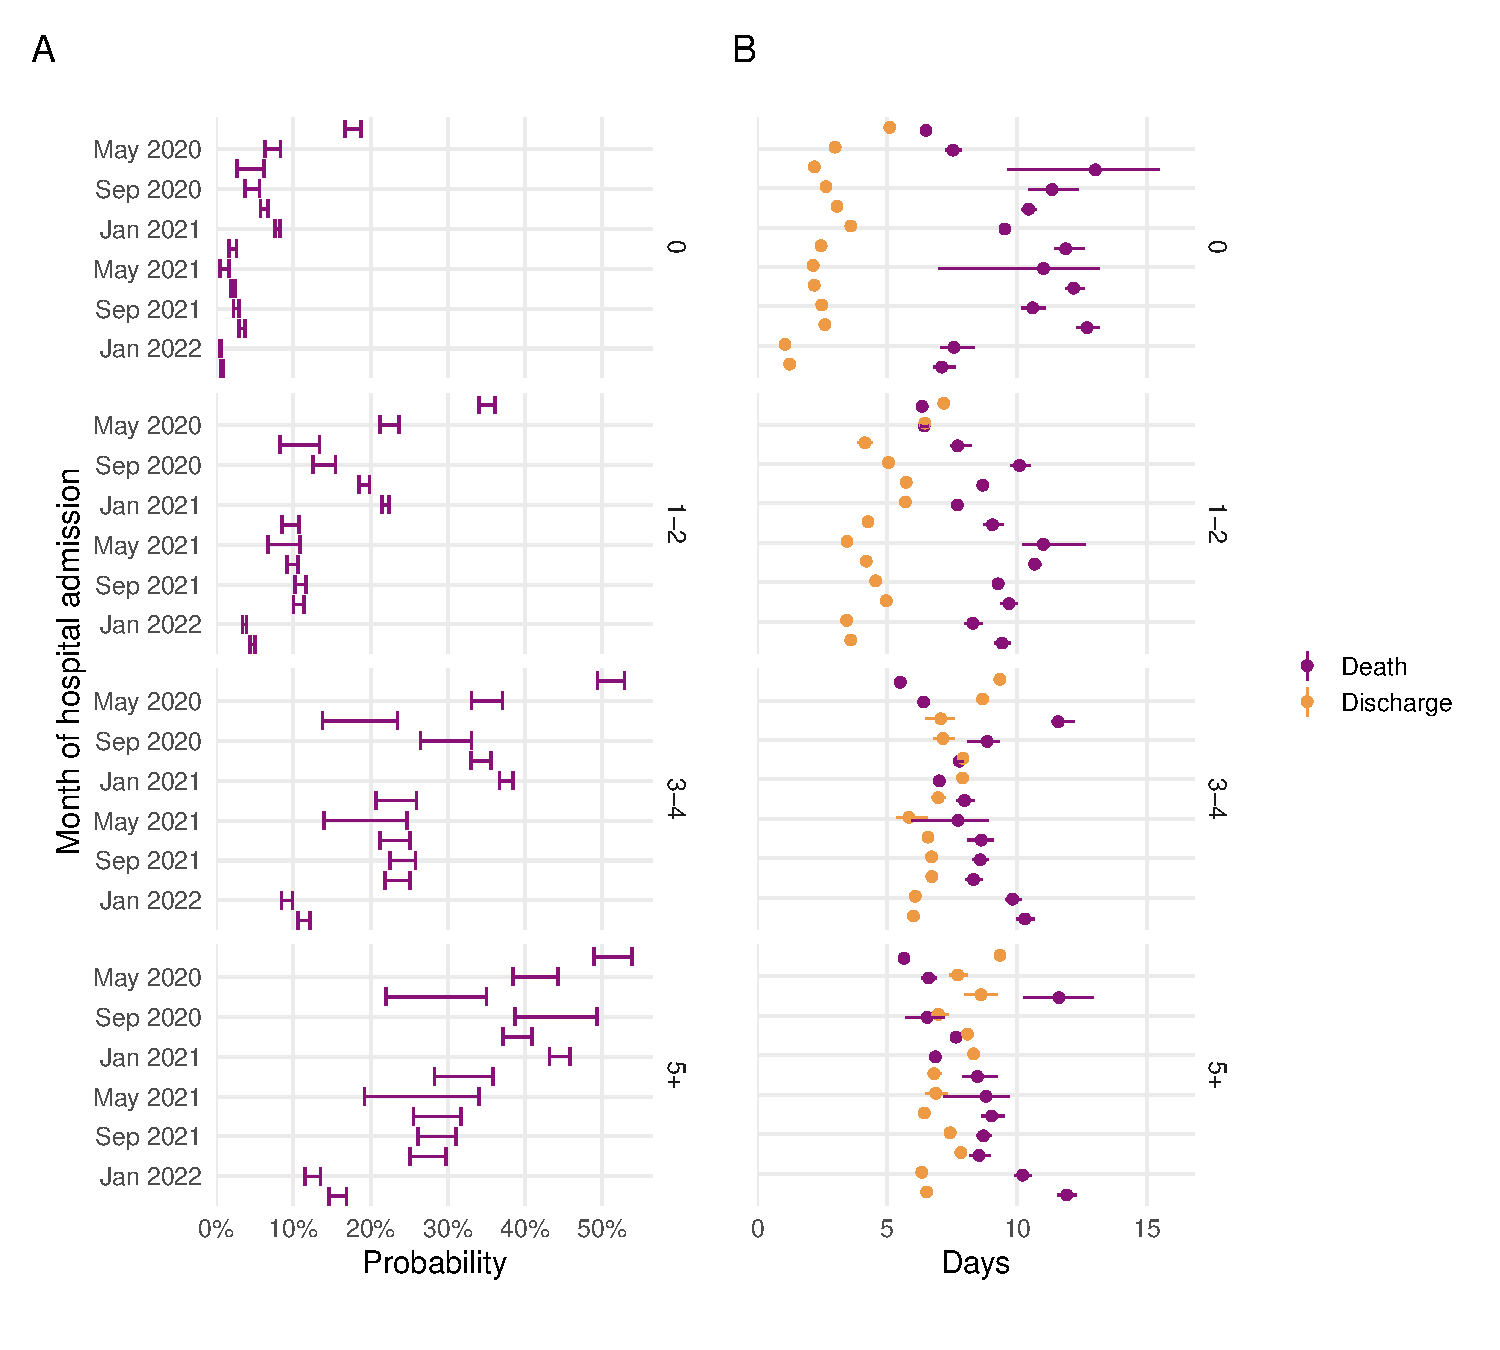
\includegraphics[width=\textwidth]{hfr_month_cci.pdf}
    \caption[Hospitalised fatality risk and median length of stay by month of admission and CCI in SUS data, March 2020 to April 2022]{Hospitalised fatality risk (panel A) and median length of stay (panel B) by month of admission and CCI in SUS data, March 2020 to April 2022. Unadjusted for other covariates. Error bars and line ranges are 95\% CIs.}\label{fig:hfr-month-cci}
\end{figure}

\begin{figure}[htbp!]
    \centering
    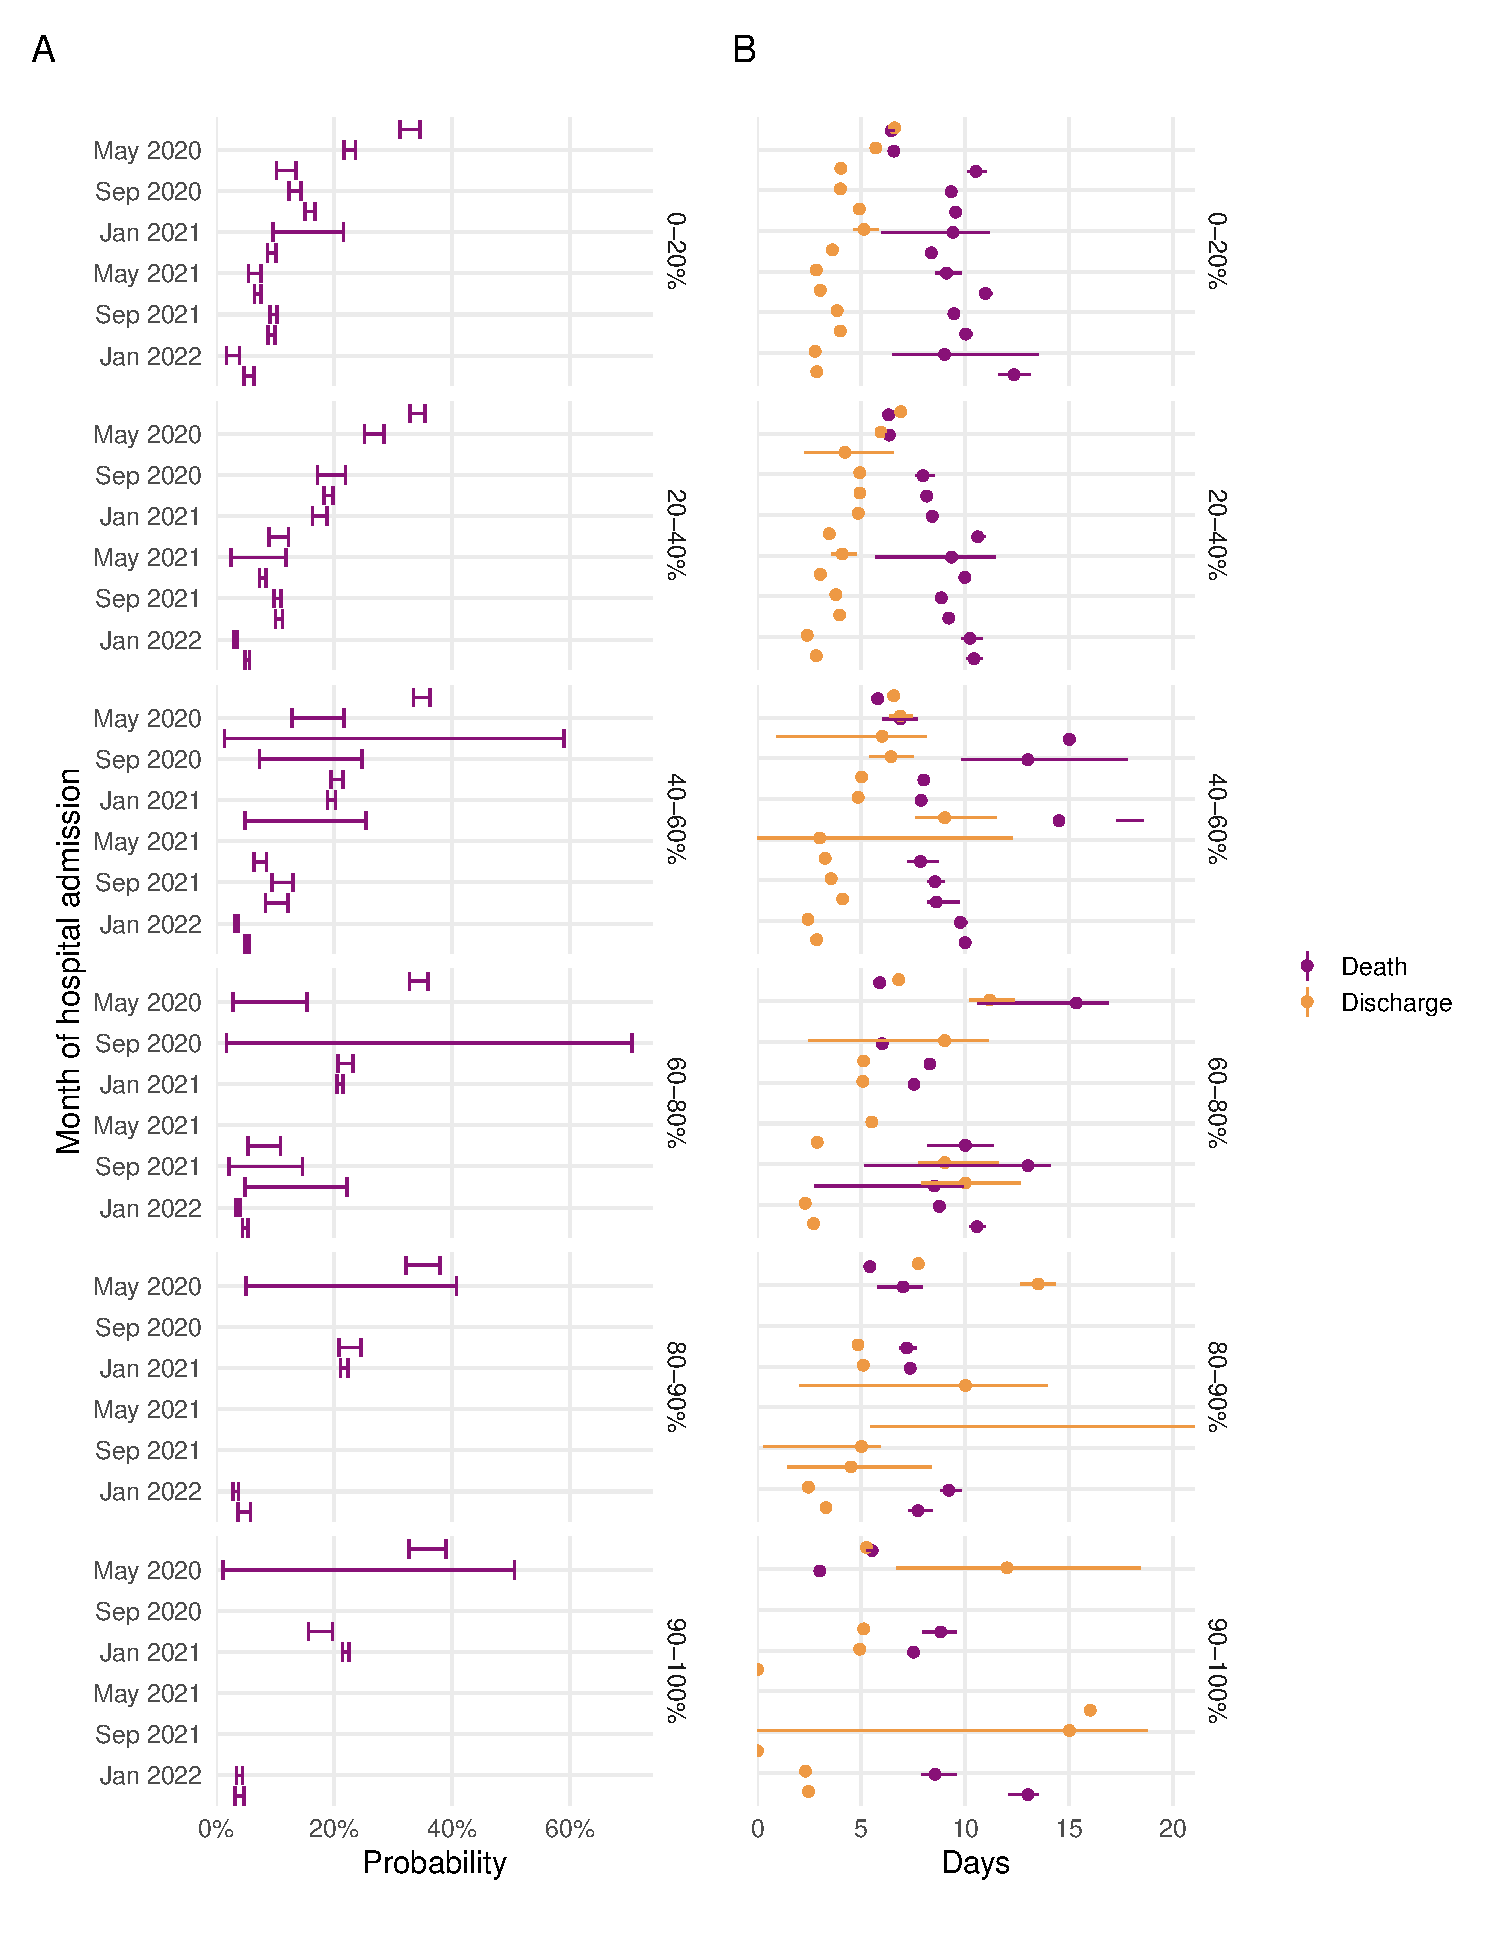
\includegraphics[width=\textwidth]{hfr_month_load.pdf}
    \caption[Hospitalised fatality risk and median length of stay by month of admission and hospital load in SUS data, March 2020 to April 2022]{Hospitalised fatality risk (panel A) and median length of stay (panel B) by month of admission and hospital load in SUS data, March 2020 to April 2022. Unadjusted for other covariates. Error bars and line ranges are 95\% CIs.}\label{fig:hfr-month-load}
\end{figure}

\begin{figure}[htbp!]
    \centering
    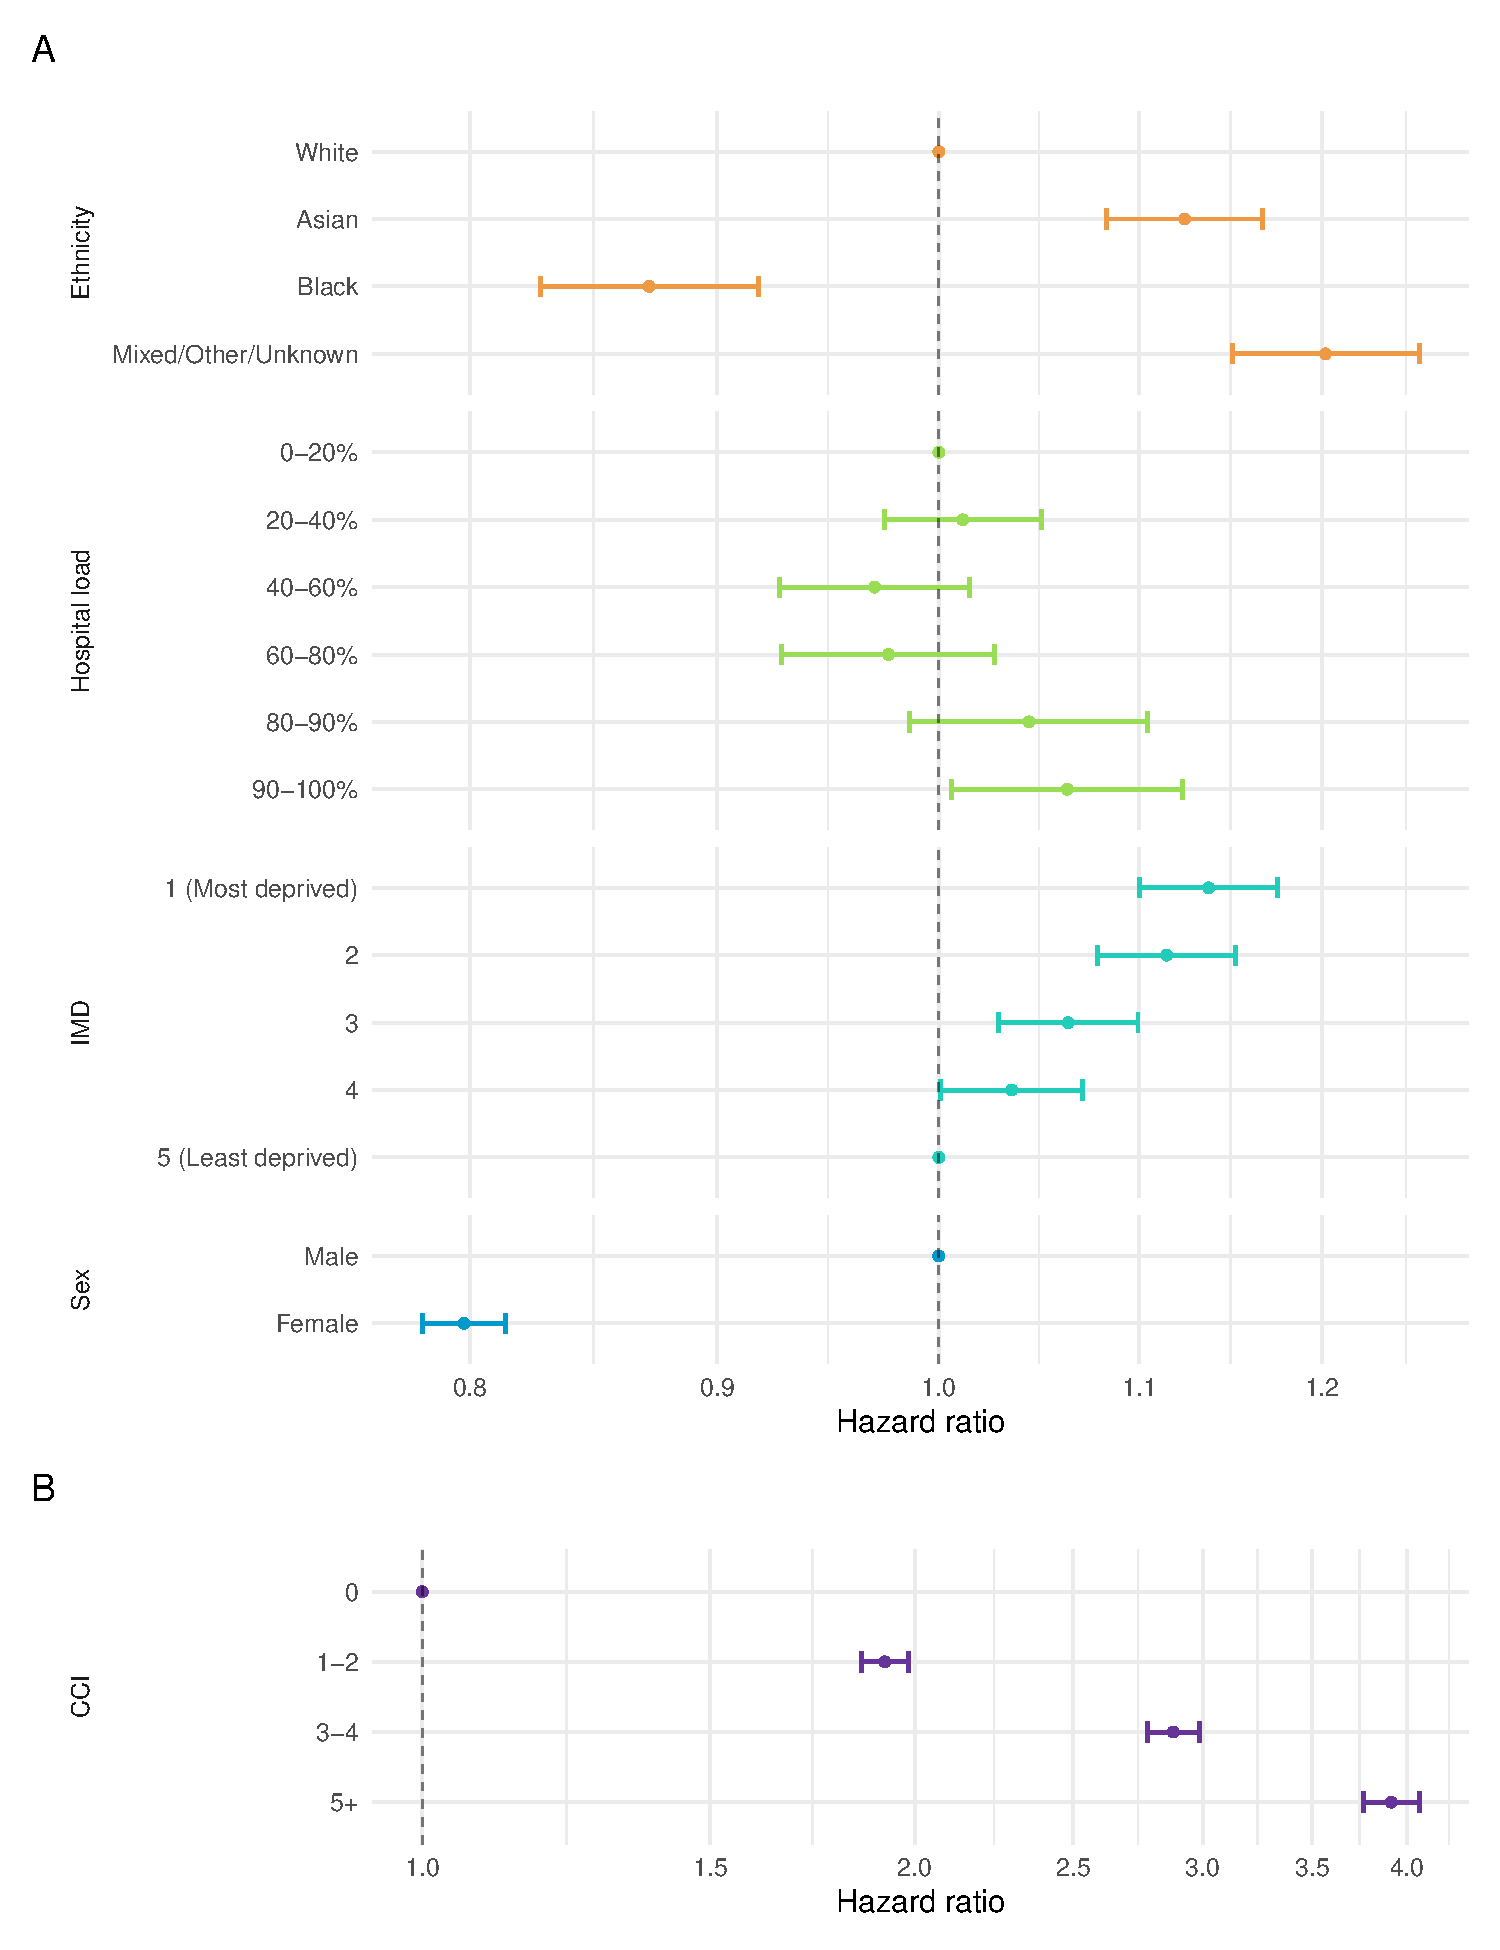
\includegraphics[width=\textwidth]{fg_hazards.pdf}
    \caption[Hospitalised fatality sub-distribution hazard ratios for sex, ethnicity, IMD quintile, hospital load and CCI in SUS data, March 2020 to April 2022]{Hospitalised fatality sub-distribution hazard ratios for sex, ethnicity, IMD quintile, hospital load and CCI in SUS data, March 2020 to April 2022. Figure shows point estimate of hazard ratio with 95\% CIs.}\label{fig:fg-hazards}
\end{figure}

\cleardoublepage

\subsection{Epidemic phase bias}\label{appendix:epi-phase-bias}

Figure~\ref{fig:fg-shift} shows the results of sensitivity analyses where the date of symptom onset was shifted later in time by $c = 0,1,2,3,4$ days for those who died, but not for those who were discharged. This model included stratification on age group, region of residence, and vaccination status, and regression adjustment on month of hospital admission, sex, ethnicity, IMD quintile, hospital load, and CCI\@.

\begin{figure}[htbp!]
    \centering
    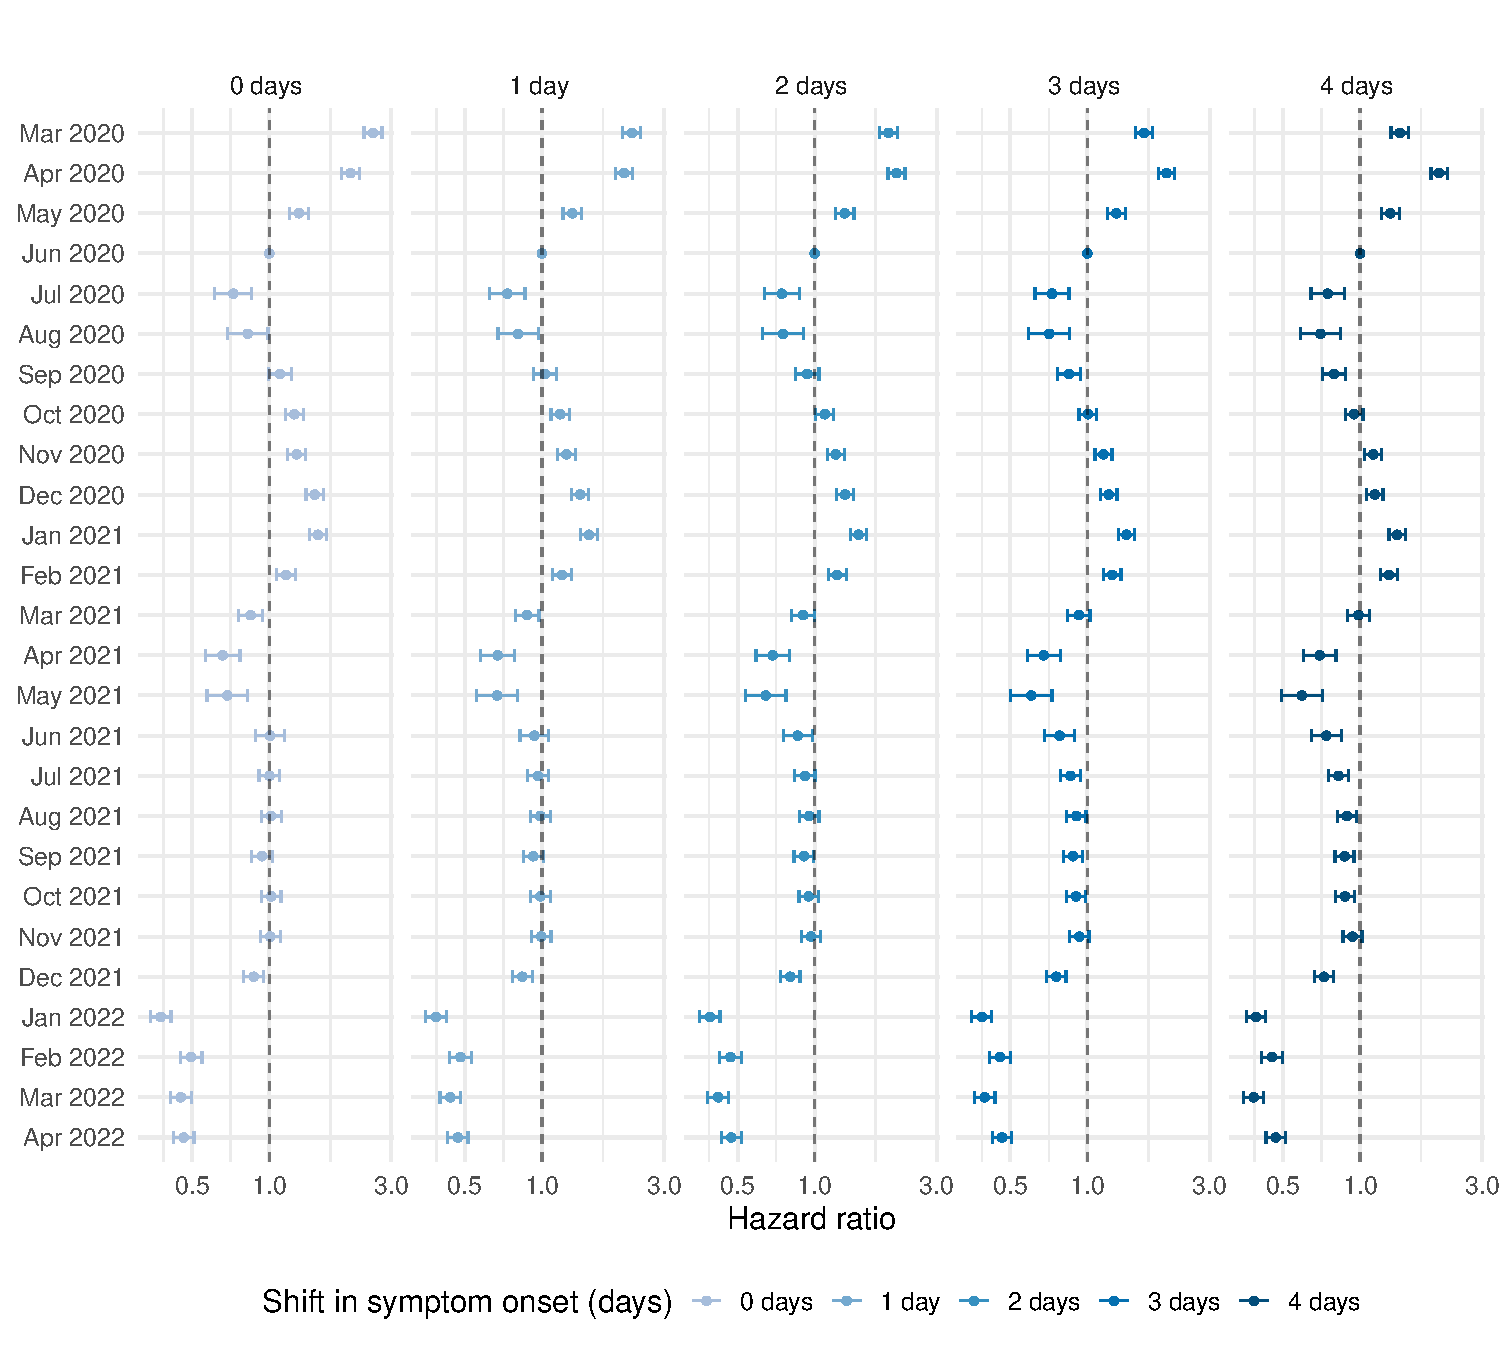
\includegraphics[width=\textwidth]{fg_shift.pdf}
    \caption[Hospitalised fatality sub-distribution hazard ratio by month of symptom onset and sensitivity in SUS data, March 2020 to April 2022]{Hospitalised fatality sub-distribution hazard ratio by month of symptom onset and sensitivity in SUS data, March 2020 to April 2022. Reference group:\ June 2020. Figure shows point estimate of hazard ratio with 95\% CIs.}\label{fig:fg-shift}
\end{figure}